\chapter{Consistent Semi-Supervised Learning on Sparse Graphs}\label{ch:SSL}

This chapter considers the consistency of graph-based semi-supervised learning methods and contextualizes the topics provided in the prints \cite{roith2022continuum, bungert2021uniform, bungert2022ratio}. We are given partially labeled data, where the task is to obtain a labeling on the  whole graph. Considering learning algorithms we are especially interested in the following aspects:
%
\begin{itemize}
\item \textbf{Consistency:} what is the behavior in the infinite data limit?
\item \textbf{Sparsity:} how does sparsity of the graph weights affect this behavior?
\end{itemize}
%
%
%
\begin{center}%
\begin{tikzpicture}
%
\hypersetup{linkcolor=black}%
\filldraw[fill=orong!20, draw=none] (0,12.5) rectangle (14.5,11.5) node[midway] {%
\cref{sec:GSSL}: \nameref{sec:GSSL}};
%\filldraw[fill=grape!20, draw=none] (0,11) rectangle (6.5,10) node[midway] {\cref{sec:pLap}: The $p$ Laplacian}; %
%\filldraw[fill=grape!10, draw=none] (0,10) rectangle (6.5,9) node[midway] {\cref{sec:pLapcont}: Continuum Setting};
%\filldraw[fill=grape!10, draw=none] (0,9) rectangle (6.5,8) node[midway] {\cref{sec:GpLap}: Graph Setting};
%
%
%
%
%
\filldraw[fill=apple!20, draw=none] (0,11) rectangle (14.5,10) 
node[midway] {\cref{sec:LipExt} Lipschitz Extensions and the Infinity Laplacian}; %
%\filldraw[fill=apple!10, draw=none] (8,10) rectangle (14.5,9) 
%node[midway] {\cref{sec:LipExtCont}: Continuum Setting}; %
%\filldraw[fill=apple!10, draw=none] (8,9) rectangle (14.5,8) 
%node[midway] {\cref{sec:GLipExt}: Graph Setting}; %
%
%
%
%
\filldraw[fill=sky!20, draw=none] (0,9.5) rectangle (7, 8.5) node[midway] {%
\cref{sec:GConv}:  \cite{roith2022continuum}};
%
\filldraw[fill=sky!20, draw=none] (7.5,9.5) rectangle (14.5, 8.5) node[midway] {%
\cref{sec:UnifConv}:  \cite{bungert2021uniform}};
%
%\filldraw[fill=sky!20, draw=none] (10,9.5) rectangle (14.5, 8.5) node[midway] {%
%\cref{sec:RatConv}:  \cite{bungert2022ratio}};
\end{tikzpicture}
\end{center}
%
In \cite{roith2022continuum} we first consider $\Gamma$-convergence of discrete $L^\infty$ functionals to their continuum counterpart. This allows to then show convergence of minimizers and therefore consistency. The proofs allow for very sparse graphs, however they only directly apply to the Lipschitz extension task, which does not allow for unique solutions. We refer to \cref{sec:GConv} for more details.

The issue of non-uniqueness is addressed in \cite{bungert2021uniform}, which considers uniform convergence of graph infinity harmonic functions to their continuum counterpart. These functions are in fact special solutions of the extension task  in \cite{roith2022continuum}, namely so-called absolutely minimizing Lipschitz extensions, which are---under certain assumptions---unique. Again, we are able to work with a very mild scaling assumption that allows for sparse graphs. Furthermore, we are able to prove the first quantitative convergence rates, where we provide the key insight, that a rate for graph distance functions transfers to a rate for infinity harmonic functions. The main contributions are presented in \cref{sec:UnifConv}.

%To allow even sparser graphs, directly at the connectivity threshold, we consider first passage percolation in \cite{bungert2022ratio}. Here, we prove a ratio convergence of a graph distance function on a Poisson point cloud. The results can ultimately be employed to show convergence rates for Lipschitz learning. Details are provided in \cref{sec:Perc}.

Before we present these works we first introduce the setting of consistency for graph-based SSL in \cref{sec:GSSL}. We then discuss the $p$-Laplacian in \cref{sec:pLap} both in the continuum and the graph setting. Similarly, we then introduce the problem we are actually concerned with namely the $\infty$-Laplacian and Lipschitz extensions in \cref{sec:LipExt}. With the necessary tools and background we are then able to present the main contributions on consistency of Lipschitz learning in the infinite data limit.
%
%
%
%
%
\section{Graph-Based SSL and Consistency}\label{sec:GSSL}

\begin{wrapfigure}{r}{.5\textwidth}
\centering
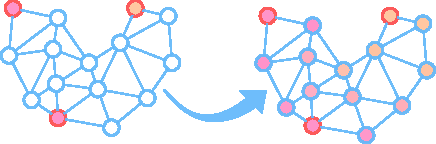
\includegraphics[width=.5\textwidth]{atelier/paradigms/GSSL.pdf}
\end{wrapfigure}

In the semi-supervised learning setting of \cref{sec:PSSL}, we are given a finite set $\domain_n\subset \tilde{\domain}$ consisting of $n$ points, where $\tilde{\domain}$ 
denotes the input space. We assume that a non-empty subset $\conset_n \subset \domain_n$ is labeled, i.e., we are given a labeling function
$\vec g:\conset_n\to\R$. From now on we denote functions acting on a discrete set $\domain_n$ using bold symbols to distinguish them from functions acting on the continuum $\tilde\domain$. In particular, the space of functions on $\domain_n$ can simply be identified with $\R^n$, since $\{\vec u:\domain_n\to\R\} \sim \R^n.$
%
\noindent%
The semi-supervised learning problem consists in finding an extension of $\vec g$ from $\conset_n$ to the whole set $\domain_n$, i.e.
%
\begin{gather}\label{eq:SSL}
\begin{gathered}\tag{SSL}
\text{find } \vec u:\domain_n\to\R,\\
\text{such that } \vec u(x) = \vec g(x) \text{ for all } x\in\conset_n.
\end{gathered}
\end{gather}
%
%
%
%
In order to obtain meaningful solutions, one usually incorporates the \emph{smoothness assumption} \cite{subramanya2014graph} which can be informally stated as follows:
%
\begin{center}
\enquote{\textit{Points that are close together are more likely to share a similar label.}}
\end{center}
%
%

\begin{remark}{Notational Remark}{}
In \cref{ch:para} we employ the symbol $\Inp$ to denote the input set, which is now replaced by $\domain$. This due to the fact, that \cite{roith2022continuum,bungert2021uniform, bungert2022ratio} employ this notation for which we choose to use it here.
\end{remark}
%
%
\noindent%
Often one assumes that the points $x\in\domain_n$ are i.i.d. w.r.t. a distribution $\mu$ with density $\rho:\domain\to\R$. However, as observed in \cite{roith2022msc}, the data distribution is not directly relevant for the works in \cite{roith2022continuum, bungert2021uniform}. The appropriate generalization to study the limit of $\domain_n$ for $n\to\infty$ is discussed in \cref{sec:GConv}.
%
%
\subsection{Weighted Graphs}
In order to employ the smoothness assumption we need a notion of \enquote{closeness} on the set $\domain_n$, for which we introduce weighted graphs. Namely we define a weighting function $w$ that allows to compare points in $\domain_n$ and therefore induces the desired notion. 
%
\begin{definition}{Weighted Graphs}{}
For a finite set $\domain_n$ and a weight function $w_n:\domain_n\times \domain_n\to\R$, the tuple $(\domain_n,w_n)$ is called a \emph{weighted graph}.
\end{definition}
%
%
\paragraph{Other Notions of Graphs}
Typically, a graph is defined as a pair $(\domain_n,E)$ where $E$ denotes the set of edges. Here, 
one has two cases:
\begin{itemize}
\item \emph{Undirected graph:} $E=\{ \{x,y\}: \text{there is an edge between } x\in \domain_n \text{ and } y\in \domain_n\}$, i.e., s
$E\subset 2^{\domain_n}$ and each edge is undirected, since $\{x,y\}=\{y,x\}$.
%
\item \emph{Directed graph:} $E=\{ (x,y): \text{there is an edge from } x \text{ to } y\}$, i.e.,
$E\subset \domain_n\times \domain_n$ and each edge is directed and $(x,y)\neq(y,x)$.
%
\end{itemize}
Additionally, one then considers a weight function $W:E\to\R$ assigning a weight to each edge, and then defines 
the triple $(\domain_n,E,W)$ as a weighted graph. However, we note that all this information can be represented much more elegantly by a weight function $w:\domain_n\times \domain_n\to\R$. A directed edge set $E\subset \domain_n\times \domain_n$ can be equivalently expressed by 
a weight function $w:\domain_n\times \domain_n\to\R$ where $w(x,y)>0$ if and only if $(x,y)\in E$, a weighting $W:E\to\R$ 
naturally transfers to $w$. In the case of an undirected graph, one simply requires the weight function to be symmetric, i.e., 
$w(x,y)=w(y,x)$ for all $x,y\in \domain_n$.
%
Furthermore, in the above definition the set $\domain_n$ does not enter the definition up to the  ordering of its $n\in \N$  elements. Therefore, a graph could be entirely represented by a weight function $w:\{1,\ldots,n\}\times\{1,\ldots,n\}\to\R$. However, since the definition of $w$ will incorporate information about points $\domain_n\subset\R^d$ we use the notation $(\domain_n, w_n)$ for graphs in the following.
%
%
%
\paragraph{Kernels and the Graph Scale} 
In most of our applications the data $\domain_n$ is given as a subset of $\R^d$ and in fact we are interested in the limit $n\to\infty$, where $\domain_n$ fills out a domain $\tilde\domain\subset\R^d$. In the continuum we consider \emph{local} operators incorporating changes of functions $u:\tilde\domain\to\R$ at an infinitesimal small scale. Since interactions on a graph are inherently non-local in the Euclidean sense, we need to localize the interaction on the graph in the limit $n\to\infty$. A popular choice that guarantees this behavior is
%
\begin{align*}
w(x,y) = \eta_{\gscale}(\abs{x-y})
\end{align*}
%
where $\eta_\gscale:[0,\infty)\to [0,\infty]$ is a kernel function depending on a scaling parameter $\gscale\in\R^+$. The parameter $\gscale$ is also referred to as the \emph{graph scale} and informally speaking determines the scale of the graph interactions. I.e., the smaller $\gscale$ the smaller the interaction radius of points in $\domain_n$ should be. In our specific setting of $L^\infty$ problems it is typical to choose
%
\begin{align*}
\eta_\gscale(\cdot) = \frac{1}{c_\eta\, \gscale} \eta\left(\frac{\cdot}{\gscale}\right)
\end{align*}
%
where $\eta$ is a non-increasing kernel and $c_\eta$ is a constant depending on the kernel. Typical examples of kernels include
%
\begin{itemize}
\item (constant weights) $\eta(t)=1_{[0,1]}(t)$,
\item (exponential weights) $\eta(t)=\exp(-t^2/(2\sigma^2))1_{[0,1]}(t)$,
\item (non-integrable weights) $\eta(t)=\frac{1}{t^p}1_{[0,1]}(t)$ with $p\in(0,1]$.
\end{itemize}
%
%
\begin{remark}{}{}
In the continuum limit one needs to consider the value 
%
\begin{align*}
\sigma_\eta = \sup_{t\in\R^+} t\, \eta(t),
\end{align*}
%
which is assumed to be finite. Considering graph problems in $L^p$ for $p<\infty$
the corresponding value is given as
%
\begin{align}\label{eq:kernelconst}
\sigma_\eta^{(p)} = \int_{\R^+} \eta(t)\, t^{d+p} dt
\end{align}
%
which was first employed in \cite{GarcSlep15} for $p=1$ and then in \cite{slepcev2019analysis} for general $p<\infty$. We see that $\sigma_\eta^{(p)}$ degenerates to $\sigma_\eta$ in the limit $p\to\infty$.

In \cite{roith2022continuum} we choose $c_\eta=1$ and therefore $\sigma_\eta$ then appears in the limit functional. In \cite{bungert2021uniform} we rescale the kernel, i.e., $c_\eta = \sigma_\eta$ which allows to work with unrescaled operators in the limit. 
\end{remark}
%
%
%
\begin{remark}{}{}
In order to obtain continuum limits in the case $p<\infty$ on usually employs a factor of $1/\gscale^{p+d}$ in front of the graph weights \cite{GarcSlep15, slepcev2019analysis}. In \cref{sec:GLipExt} we see that this factor degenerates to $1/\gscale$ in the case $p\to\infty$. The intuition here, is that problems in $L^\infty$ do not respect mass in a quantitative but rather a qualitative manner. Therefore, factors like $\gscale^d$ which appear because of integrals in $\R^d$ do not contribute for $p=\infty$.
\end{remark}
%
%
\paragraph{Sparse Graphs}
An important practical aspect connected to the graph scale is the sparsity of the graph, which is given by the numbers of non-zero elements in the weight matrix $W\in\R^{n\times n}$
%
\begin{align*}
W_{ij}:= w(x_i,x_j) \quad x_i,x_j\in\domain_n
\end{align*}
%
where we assume an ordering $\domain_n=\{x_1,\ldots, x_n\}$. In order to have a computationally feasible problem this matrix should have very few non-zero elements. Assuming that the kernel $\eta$ has compact support, w.l.o.g. $\supp(\eta)\subset [0,1]$ we observe that the sparsity is directly influenced by the graph scale $\gscale$. Namely, $\abs{x_i-x_j} > \gscale \Rightarrow W_{ij}=0$, see \cref{fig:graphscale}.
%
%
\begin{figure}
\centering
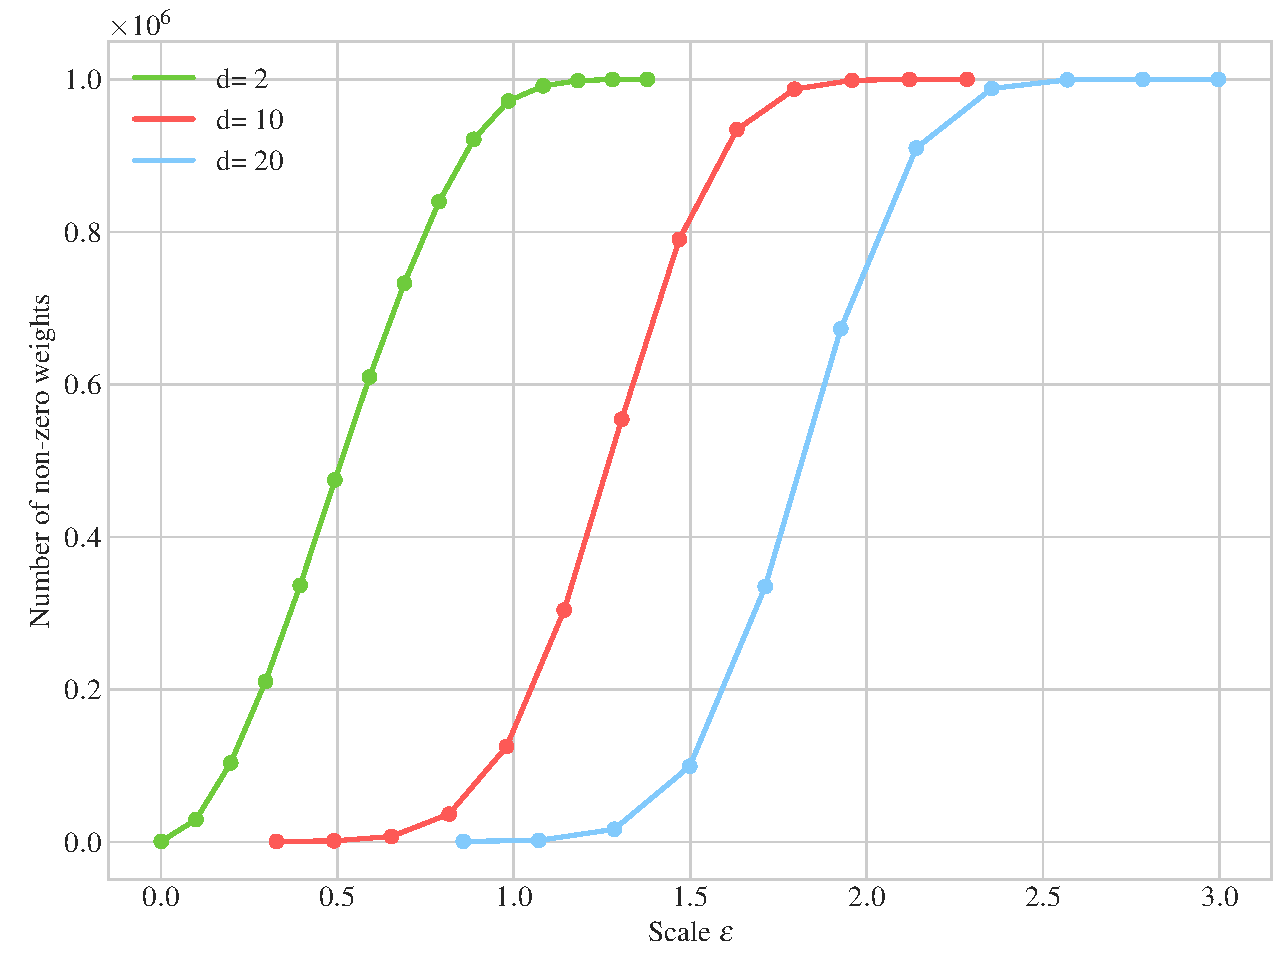
\includegraphics[width=.5\textwidth]{code/SSL/NNZ.pdf}
\caption[Dependence of the number of non-zero edges on the scaling parameter $\gscale$.]{Dependence of the number of non-zero edges on the scaling parameter $\gscale$. Here, we sample $n\in\N$ points uniformly in the cube $[0,1]^d$ and only connect vertices $x_i,x_j\in\domain_n$ if $\norm{x_i-x_j}_2 < \gscale$. The plots shows the behavior for $d=2,10,20$.}\label{fig:graphscale}
\end{figure} 
%
%
Therefore, from a practical point of view $\gscale$ should be chosen relatively small. However, showing consistency of graph-based SSl algorithms often requires scaling assumptions that permit the desired length scales \cite{GarcSlep15, slepcev2019analysis, calder2019consistency}. In \cref{sec:GConv} we give concrete examples of such scaling assumptions. One of the main goals of \cite{roith2022continuum, bungert2021uniform} was to show convergence and rates at the smallest possible length scale, which was indeed achieved.
%
%
%
\begin{remark}{}{}
In many practical applications graph weights connecting all points within $\gscale$-ball of Euclidean distance are inferior to knn graphs \cite{calder2020poisson, flores2019algorithms, calder2022improved}. While most consistency results employ the $\gscale$-ball setting, recently, the authors in \cite{calder2022improved} were able to show convergence rates in the knn setting. In this thesis we focus on the $\gscale$-ball setting, however it is an interesting open question to transfer the results of \cite{roith2022continuum, bungert2021uniform, bungert2022ratio} to the knn setting.
\end{remark}
%
%
%
%
\subsection{The $p$-Laplacian: Continuum and Graph}\label{sec:pLap}
%
%
The archetype of learning methods we consider in the following is so-called \emph{Laplacian learning}, which had one of its first appearances in 
\cite{zhu2003semi}. The associated problem was given as
%
\begin{gather}\label{eq:SSL_Laplacian}
	\begin{gathered}
		\min_{\vec u:\domain_n\to\R} \sum_{x,y\in\domain_n} w_n(x,y)^2 
		\left(\vec u(y) - \vec u(x) \right)^2\\
		\text{subject to } \vec u(x) = \vec g(x) \text{ for all } x\in\conset_n.
	\end{gathered}
\end{gather}
%
%
%
Here, we always assume non-negative weights $w_n:\domain_n\times\domain_n\to[0,\infty)$. The intuitive idea behind this method is that it minimizes a discrete approximation of the Dirichlet energy and should therefore enforce a certain kind of \enquote{smoothness} of the solution $\vec u$. In \cite{zhou2005regularization} it was proposed to generalize the idea of the graph Dirichlet energy in \cref{eq:SSL_Laplacian} to arbitrary $1\leq p < \infty$ motivated by the continuum counterpart. While The contributions in \cite{roith2022continuum, bungert2021uniform, bungert2022ratio} mainly consider the case of $p=\infty$, the case $p<\infty$ serves as a  motivation for the whole discussion. Therefore, we briefly review the situation in the following. Here, we first introduce the continuum setting and then discuss the situation on the graph.
%
%
%
%
\paragraph{Continuum Setting}
We follow the exposition in \cite{lindqvist2017notes}. Let $\domain\subset\R^d$ be a bounded domain, then we consider the $p$-Dirichlet energy for functions $u\in W^{1,p}(\domain)$,
%
\begin{align}\label{eq:DirichletEnergy}
	\pDir{}_{p,\rho}(u) := \int_\domain \abs{\nabla u}^p \rho(x)^2 \, dx,
\end{align}
%
%
where $\rho:\domain\to\R$ is some given function. In the setting of \cite{GarcSlep15, slepcev2019analysis} $\rho$ denotes the density of data distribution as in \cref{sec:GSSL}. For $\rho\equiv1$ we simply write $\pDir{}_{p,1}=\pDir{}_{p}$. The associated variational problem is given in the following.
%
\begin{problem}{Variational Formulation}{prob:VarForm}
	For $p\in (1,\infty)$ and $V\subset W^{1,p}(\domain)$ find $u\in W^{1,p}(\domain)$ such that
	%
	\begin{align*}
		\pDir{}_{p,\rho}(u) \leq \pDir{}_{p,\rho}(v)
	\end{align*}
	%
	for all $v$, such that $(u-v)\in W^{1,p}_0$.
\end{problem}
%
\noindent%
Assume for simplicity that $\rho\equiv 1$ and that $u\in V$ is a minimizer of the above problem, then its first variation must vanish, i.e., for all $\phi\in C^\infty_0(\domain)$ one has
%
\begin{align}\label{eq:weakLap}
	\int_\domain \langle \abs{\nabla u}^p \nabla u, \nabla \phi \rangle \, dx = 0.
\end{align}
%
A function $u\in V$ satisfying \cref{eq:weakLap} is called a \emph{weak solution} of the $p$-Laplace equation. In fact, if $u$ 
is smooth enough one has that
%
\begin{align}\label{eq:strongLap}
	\Delta_p u := \div(\abs{\nabla u}^{p-2} \nabla u) = 0
\end{align}
%
where $\Delta_p$ is called the $p$-Laplacian. Boundary conditions on $\partial \domain$ given by a function $g\in W^{1,p}(\domain)$  can be incorporated by considering the set
$V_g := \{u\in W^{1,p}(\domain): u-g \in W^{1,p}_0(\domain)\}$. 
We state the following classical result, which can for example be found in \cite{lindqvist2017notes}.
%
\begin{theorem}{Existence and Uniqueness}{}
	For $p\in (1,\infty)$ and $g\in W^{1,p}(\domain)$ there exists a unique minimizer $u\in V_g$ of the $p$-Dirichlet energy, i.e.,
	%
	\begin{align*}
		\argmin_{u\in V_g} \pDir{}_p(u) = u.
	\end{align*}
	%
	Moreover, $u$ is a weak solution of the $p$-Laplace equation and there exists a function $\tilde{u}\in C(\domain)$ such that
	$u = \tilde{u}$ a.e. in $\domain$. If $g\in C(\domain)$ and $\domain$ is sufficiently smooth, then 
	$\tilde{u}\vert_{\partial \domain} = g\vert_{\partial \domain}$.
\end{theorem}
%
%
\begin{proof}
	The proof can be found in \cite[Thm. 2.16]{lindqvist2017notes}.
\end{proof}
%
%
\paragraph*{Local Minimization Property} Let $u$ solve \cref{prob:VarForm} for given boundary values $g\in W^{1,p}(\domain)$ and let $V\subset\subset\domain$ be a sufficiently regular subset. Then we have that
%
\begin{align*}
\pDir_p(u) = \int_{V} \abs{\nabla u}^p dx + \int_{\domain\setminus V} \abs{\nabla u}^p dx.
\end{align*}
%
Now consider \cref{prob:VarForm} on $V$ with boundary values given by $u$ and denote by $v$ the solution of the problem. Since $u=v$ on $\partial V$ we can extend $v$ onto $\domain$ by setting $v=u$ in $\domain\setminus V$, which gives $v\in W^{1,p}(\domain)$. Therefore, we obtain
%
\begin{align*}
\pDir_p(v) = \int_{V} \abs{\nabla v}^p dx + \int_{\domain\setminus V} \abs{\nabla u}^p dx \leq 
\int_{V} \abs{\nabla u}^p dx + \int_{\domain\setminus V} \abs{\nabla u}^p dx = \pDir_p(u).
\end{align*}
%
Since $u$ was unique this yields $u|_V = v|_V$, and therefore we know that any solution on $\domain$ solves \cref{prob:VarForm} also on any \enquote{nice} subset, with the boundary values given by itself. In \cref{sec:LipExt} we see that this \textit{local minimization property} does not hold automatically and has to enforced additionally. The underlying reason here is, that integrals are set-additive, but suprema are not, which is similarly explained in \cite{aronsson2004tour}.

%
%
\paragraph{Laplacian Learning} A natural extension of the problem given in \cref{eq:DirichletEnergy} is obtained by considering the target functional
%
\begin{align*}
	\GE^{w_n}_p(\vec u):= \sum_{x,y\in\domain_n} w_n(x,y)^p \abs{\vec u(y) - \vec u(x)}^p,
\end{align*}
%
which we refer to as the graph $p$-Dirichlet energy. Indeed, we notice structural 
similarities to the $p$-Dirichlet energy $\pDir_p$ in \cref{eq:DirichletEnergy}, replacing the integral by a finite 
sum and derivatives by weighted finite differences
%
\begin{align*}
	w_n(x,y)^p \abs{\vec u(y) - \vec u(x)}^p.
\end{align*}
%
This naturally leads to the following minimization problem.
%
\begin{problem}{Graph Energy Minimization}{prob:vargraph}
Given a weighted graph $(\domain_n, w_n)$ and a labeling function $\vec g:\conset_n\to\R$, for $\conset_n\subset\domain_n$ we consider 
the problem
%
\begin{align*}
	\min_{\vec u:\domain_n\to\R} \GE^{w_n}_p(\vec u) \text{ subject to } \vec u(x) = \vec g(x) \text{ for all } x\in\conset_n.
\end{align*}
\end{problem}
%
\noindent%
Since every function $\vec u:\domain_n\to\R$ can be identified with a vector $\vec u\in\R^n$, the above problem 
is in fact an optimization problem in $\R^n$. The functional $\GE^{w_n}_p:\R^n\to\R$ is bounded from below by $0$, continuous, convex and in the case $p>1$ even differentiable. However, one can prove unique existence with techniques very similar to the continuum case in \cite{lindqvist2017notes}. We give the adapted prove below for completeness. The important property to establish uniqueness is that the graph is connected to the boundary, i.e., for every $x\in\domain_n$ there exists a path $x=\gamma_1,\ldots,\gamma_m=o\in\domain_n$ with $w(\gamma_{i+1}, \gamma_i)>0$ connecting $x$ to a point $o\in\conset_n$ in the boundary. This is very intuitive, since on any connected component that does not communicate with the boundary, an arbitrary constant minimizes the \enquote{graph gradient}.
%
%
\begin{theorem}{Existence and Uniqueness}{} Let $(\domain_n,w_n)$ be a graph with non-negative weights, that is connected to its boundary $\conset_n\subset\domain_n$. Then \cref{prob:vargraph} admits a unique solution $\vec u:\domain_n\to\R$.
\end{theorem}
%
\begin{proof}
The	proof is an adaption from the continuum case in \cite[Thm. 2.16]{lindqvist2017notes}. We start by proving uniqueness, 	
Let $E = \{(x,y): w_n(x,y)>0\}$ be the set of all active edges and denote by $\nabla^{w_n} \vec u \in \R^{\abs{E}}$
%
\begin{align*}
(\nabla^{w_n} \vec u)_{(x,y)} := w_n(x,y) \left(\vec u(y) - \vec u(x)\right)
\end{align*}
%
the \enquote{graph gradient} on $E$, where we have that
%
\begin{align*}
\GE^{w_n}_p (\vec u) = \sum_{(x,y)\in E} w_n(x,y)^p \abs{\vec u(y) - \vec u(x)}^p 
= \sum_{(x,y)\in E} \abs{(\nabla^{w_n} \vec u)_{(x,y)}}^p=
\norm{\nabla^{w_n}\vec u}_p^p.	
\end{align*}
%
%
Let $\vec u_1, \vec u_2$ be two  solutions of \cref{prob:vargraph}, i.e. $\GE^{w_n}_p (\vec u_1)= \GE^{w_n}_p (\vec u_2)$. Since $\vec u_1,\vec u_2$ fulfill the boundary conditions, this also holds for $1/2(\vec u_1 + \vec u_2)$ and therefore $\GE^{w_n}_p(\vec u_1)\leq\GE^{w_n}_p(1/2(\vec u_1 + \vec u_2))$.


Assume that there exists $(\bar x,\bar y)\in E$ such that $\nabla^{w_n} \vec u_1(\bar x,\bar y)\neq \nabla^{w_n}\vec u_2(\bar x,\bar y)$, then we have that
%
\begin{align*}
\GE^{w_n}_p (\vec u_1) &\leq \GE^{w_n}_p \left(\frac{\vec u_1 + \vec u_2}{2}\right) =
\norm{\frac{\nabla^{w_n} \vec u_1(x,y) + \nabla^{w_n} \vec u_2(x,y)}{2}}^p_p\\
&<
\frac{1}{2} \sum_{(x,y)\in E\setminus\{(\bar x,\bar y)\}} \abs{\nabla^{w_n} \vec u_1(x,y)}^p + \abs{\nabla^{w_n} \vec u_2(x,y)}^p
\\ 
&\qquad+\frac{1}{2} \abs{\nabla^{w_n} \vec u_1(\bar x, \bar y)}^p + \abs{\nabla^{w_n} \vec u_2(\bar x, \bar y)}^p\\
&= 
\frac{1}{2}\left(\GE^{w_n}_p (\vec u_1) + \GE^{w_n}_p (\vec u_2)\right) 
= \GE^{w_n}_p (\vec u_1),
\end{align*}
%
which is a contradiction. Here, we employed the strict convexity of $t\mapsto \abs{t}^p$ which implies $\abs{t+\bar t}^p \leq 2^{p-1} \left(\abs{t}^p + \abs{\bar t}^{p}\right)$, where the inequality is sharp if $t\neq \bar t$. Therefore, we obtain that $\nabla^{w_n} \vec u_1 = \nabla^{w_n}\vec u_2$, which yields
%
\begin{align}\label{eq:diffid}
\vec u_1(y) - \vec u_1(x) = \vec u_2(y) - \vec u_2(x) \qquad\text{for all}\qquad (x,y)\in E.
\end{align}
%
Since $(\domain_n, w_n)$ is connected to $\conset_n$ for any $x\in\domain_n$ we can find a path $x=\gamma_1,\ldots,\gamma_m=o$ connecting $x$ to a point $o\in\conset_n$. By definition $w_n(\gamma_{i+1}, \gamma_i) >0$ for all $i=1,\ldots, m-1$ and therefore using \cref{eq:diffid} we obtain
%
\begin{align*}
\vec u_1(\gamma_{i}) - \vec u_1(\gamma_{i+1}) = \vec u_2(\gamma_{i}) - \vec u_2(\gamma_{i+1}) \qquad\text{for all}\qquad i=1,\ldots,m-1.
\end{align*}
%
which together with the boundary conditions $\vec u_1(o)=\vec u_2(o)=\vec g(o)$ yields
%
\begin{align*}
\vec u_1(x) = 
\vec u_1(\gamma_1)= \vec u_1(\gamma_1) &- \vec u_1(\gamma_2) + \vec u_1(\gamma_2)\\
%
=\ldots=\Bigg[\sum_{i=1}^{m-1} \vec u_1(\gamma_{i}) &- \vec u_1(\gamma_{i+1})\Bigg] + 
\vec u_1(o)\\
= \Bigg[\sum_{i=1}^{m-1} \vec u_2(\gamma_{i}) &- \vec u_2(\gamma_{i+1})\Bigg] + 
\vec u_2(o)\\
%
=\vec u_2(x)\phantom{---}&
\end{align*}
%
Since $x\in\domain_n$ was arbitrary, we get $\vec u_1 = \vec u_2$.\par
%
\noindent%
To show existence, we do not need to assume that the graph is connected to the boundary. On every connected component $V\subset \domain_n$ that is not connected to $\conset$ we can set $\vec u(x) = c$ for all $x\in V$, where $c\in\R$ is an arbitrary constant. We can select all edges in $V$, i.e. $E_V := E \cap V^{\times 2}$ and since $V$ was a connected component---i.e. it does not have active edges to vertices outside of $V$---we can also split up the functional
%
\begin{align*}
\GE^{w_n}_{p}(\vec u) = \sum_{(x,y)\in E\setminus E_V} \abs{\nabla^{w_n} \vec u(x,y)}^p
+
\underbrace{\sum_{(x,y)\in E_V} \abs{\nabla^{w_n} \vec u(x,y)}^p}_{=0} = 
\sum_{(x,y)\in E\setminus E_V} \abs{\nabla^{w_n} \vec u(x,y)}^p
\end{align*}
%
where the contribution on the connected component is zero, since we set $\vec u$ to be constant here. Therefore, w.l.o.g. we can assume that $\domain_n$ is connected to the boundary, since any component not connected to boundary does not contribute to the problem. Let now $\vec u:\domain_n\to\R$ be a function and for $x\in\domain_n$ let $\gamma \in \domain_n^{\times m}$ be a path to a point in the boundary $o^x\in\conset_n$, then we have that
%
\begin{gather*}
\abs{\vec u(x)}^p \leq C\left(\sum_{i=1}^{m^x-1}\abs{\vec u(\gamma_{i}) - \vec u(\gamma_{i+1})}^p + \abs{\vec g(o^x)}^p\right) \leq 
C\left(\GE^{w_n}_p(\vec u) + \abs{\vec g(o^x)}^p\right)
\end{gather*}
%
where $C>0$ is a generic constant---not depending on $\vec u$---that also accounts for the factor $\left(\min_{(x,y)\in E}w_n(x,y)\right)^{-1}$. Summing over all $x\in\domain_n$ yields

\begin{gather*}
\norm{\vec u}^p_p = \sum_{x\in\domain_n} \abs{\vec u(x)}^p \leq 
C\left( n\, \GE^{w_n}_p(\vec u) + \sum_{x\in\domain_n} \abs{\vec g(o^x)}^p\right)\\
%
\leq  C \bigg(\GE^{w_n}_p(\vec u) + \norm{\vec g}^p_p\bigg).
\end{gather*}
%
Let now $\vec u_j$ denote a sequence such that
%
\begin{align*}
\GE^{w_n}_p(\vec u_j) \leq I + 1/j,\qquad\text{ where }\qquad
I := \inf_{\vec u=\vec g\text{ on } \conset_n} \GE^{w_n}_p(\vec u).
\end{align*}
%
Then we have that
%
\begin{align*}
\norm{\vec u_j}^p_p \leq C\ (\GE^{w_n}_p(\vec u_j) + \norm{\vec g}^p_p)
\leq C\ (I + 1/j + \norm{\vec g}^p_p) \leq \tilde C
\end{align*}
%
$j\in\N$, i.e. $\vec u_j$ is a uniformly bounded sequence of vectors in the finite dimensional space $\R^n$, and therefore there exists a subsequence---which we do not relabel---that converges to some $\vec u^\ast\in\R^n$. Since the functional $\GE^{w_n}_p:\R^n\to\R$ is continuous we obtain that
%
\begin{align*}
\GE^{w_n}_p(\vec u^\ast) = \lim_{j\to\infty} \GE^{w_n}_p(\vec u_j) = I
\end{align*}
%
which yields existence.
\end{proof}
%
%
\paragraph{The Graph Laplacian}
%
In the continuum case one considers the Euler--Lagrange equation for the functional $\pDir_p$, which yields the 
$p$-Laplacian, see \cref{sec:pLap}. Analogously, the optimality conditions for the graph $p$-Dirichlet energy $\GE^{w_n}_p:\R^n\to\R$ for $p > 1$ yield
%
\begin{align*}
\nabla_{\vec u} \GE^{w_n}_p(\vec u) = 0
\end{align*}
%
where for $x\in\domain_n$ we have 
\begin{align*}
\left(\nabla_{\vec u} \GE^{w_n}_p(\vec u)\right)_x =:\Delta^{w_n}_p \vec u(x)= \sum_{y\in\domain_n} w_n(x,y)^p \abs{\vec u(y) - \vec u(x)}^{p-2} \left( \vec u(y) - \vec u(x) \right)
\end{align*}
%
which is referred to as the graph $p$-Laplacian operator. This yields the following problem.
%
\begin{problem}{Graph $p$-Laplacian}{prob:graphLaplace}
	Given a weighted graph $(\domain_n, w_n)$ and a labeling function $\vec g:\conset_n\to\R$ with $\conset_n\subset\domain_n$, find 
	a function $\vec u:\domain_n\to\R$ such that
	%
	\begin{align*}
		\Delta_p^{w_n} \vec u &= 0, \text{ in } \domain_n\setminus \conset_n,\\
		\vec u &= \vec g \text{ on } \conset_n.
	\end{align*}
\end{problem}
%
\noindent%
Since the functional $\GE^{w_n}_p$ has a unique minimizer subject to the constraints given by $\vec g$ and the graph $p$-Laplacian is derived 
via optimality conditions, one expects that the \cref{prob:vargraph} and \cref{prob:graphLaplace} are equivalent. This is formulated in the following 
theorem.
%
\begin{theorem}{Existence and Uniqueness}{}
Let $(\domain_n,w_n)$ be a graph with non-negative weights, that is connected to its boundary $\conset_n\subset\domain_n$. Then there exists a unique solution $\vec u:\domain_n\to\R$ to \cref{prob:graphLaplace}, which also is the unique minimizer of \cref{prob:vargraph}.
\end{theorem}
%
\begin{proof}
This statement can be proven similarly to \cite[Theorem 5.3]{elmoataz2015p}.
\end{proof}
%
%
%
%
%
\subsection{Consistency for Graph-based SSL}\label{sec:CSSL}
%
%
While the graph 2-Laplacian has been successfully employed for classification tasks, see e.g. \cite{zhu2003semi, zhou2005regularization}, it has been observed that solutions tend to degenerate for large amounts of data, whenever $d\geq 2$ \cite{nadler2009statistical, alamgir2011phase, el2016asymptotic}. We illustrate this phenomenon in \cref{ex:pLapBad}.
%
\begin{figure}
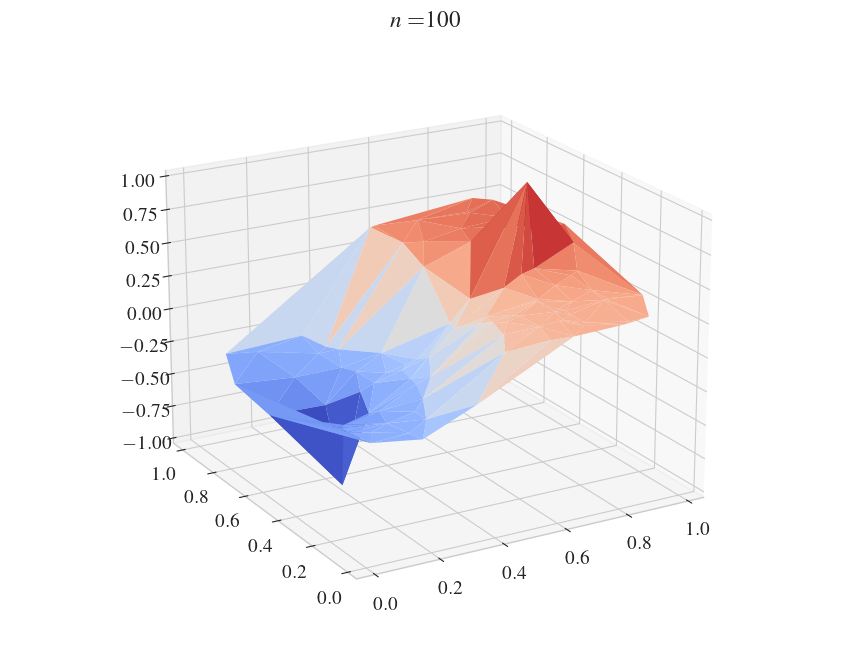
\includegraphics[width=.28\textwidth, trim={3.1cm 1cm 3.5cm 0cm},clip]{code/SSL/2Dex_100.png}%
\hfill%
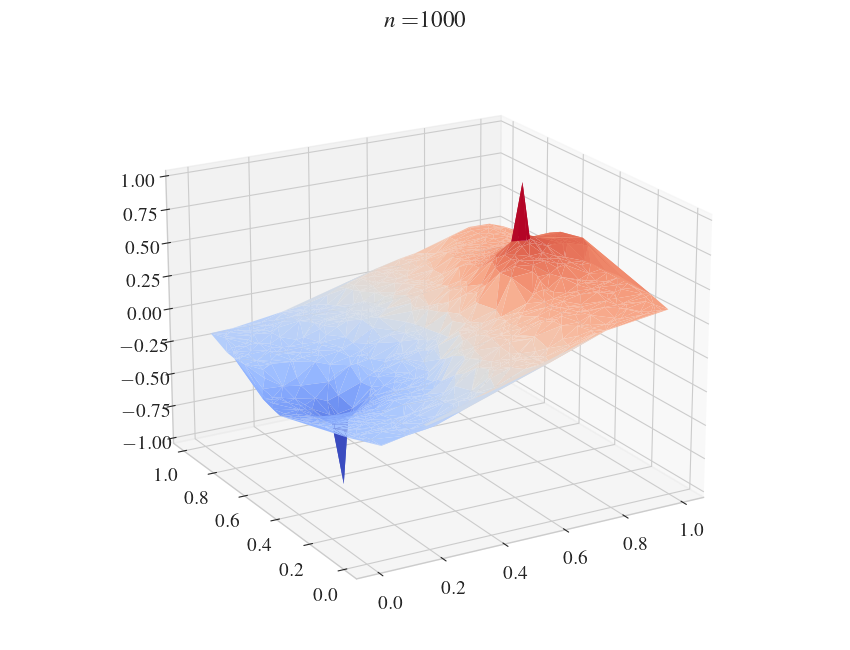
\includegraphics[width=.28\textwidth,trim={3.1cm 1cm 3.5cm 0cm},clip]{code/SSL/2Dex_1000.png}%
\hfill%
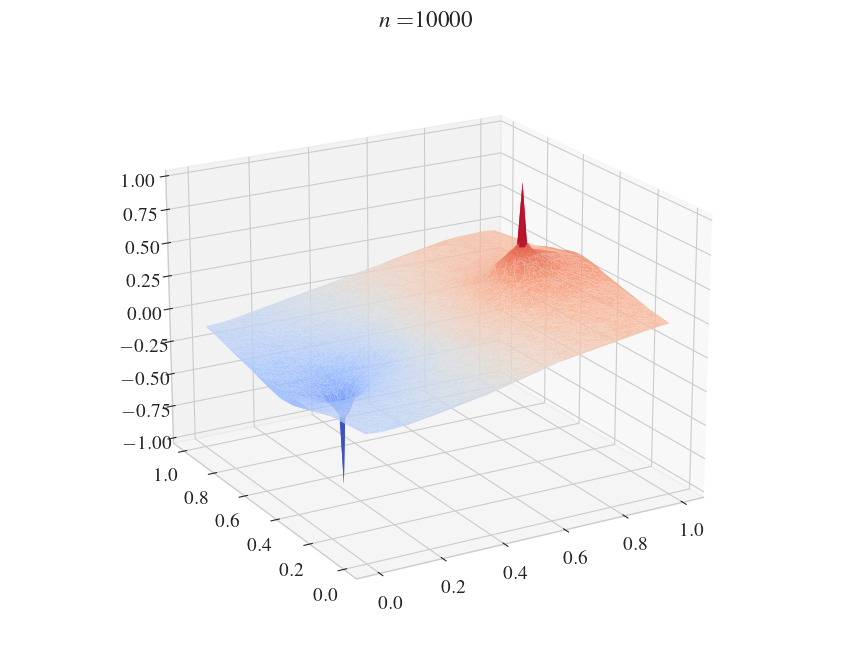
\includegraphics[width=.28\textwidth,trim={3.1cm 1cm 3.5cm 0cm},clip]{code/SSL/2Dex_10000.png}%
%
\caption[Solution to the Laplacian Learning problem for different number of data points.]{Solution to the Laplacian Learning problem ($p=2$) for different number of data points $n\in\{100,1000,10000\}$.}\label{fig:pdeg}
\end{figure}
%
%
\begin{example}{}{ex:pLapBad}
We sample different number of points $n\in\{100,1000,10000\}$ in $(0,1)^2$ and keep a fixed constraint on $\conset_n=\{o_1, o_2\}=\{(0.2,0.5), (0.8, 0.5)\}$ with $\vec g(o_1) = -1, \vec g(o_2)=1$. In \cref{fig:pdeg} we observe that for increasing $n$ the solution $\vec u$ of \cref{eq:SSL_Laplacian} tends to be a constant equal to the average of the given constraints and spike at the given constraints.
\end{example}
%
%
\noindent%
This observation motivates the driving question of this chapter and the works presented:
%
\begin{center}
\textit{%
Are Semi-Supervised Learning algorithms consistent in the infinite data limit?}
\end{center}
%
In our case \enquote{consistency} roughly ask the discrete solutions to converge to the continuum counterparts they are motivated by, in the data limit $n\to\infty$. Here, we distinguish between point-wise consistency as in \cite{von2008consistency, gine2006empirical, hein2005graphs}, consistency on a function space level \cite{slepcev2019analysis, GarcSlep15,calder2019consistency, roith2022continuum, bungert2021uniform} and consistency of a discretized operator \cite{calder2019consistency, bungert2022ratio}. Other related work also consider the limit of clustering methods \cite{hoffmann2022spectral, trillos2018variational} or the no-noise limit \cite{hoffmann2020consistency, dunlop2020large}. We detail the notion of consistency in the following.  
%
%
\paragraph{Consistency for the $p$-Laplacian} 
As observed in \cite{nadler2009statistical, alamgir2011phase, el2016asymptotic, calder2020properly} the question of consistency is now connected to the relation between $p$ and $d$, where one considers the three regimes $p<d$, $p=d$ and probably the most relevant case $p>d$. The $p$-Dirichlet problem in the continuum can be formulated as a variational problem in $W^{1,p}$. However, it is important to remember that in our setting we most likely consider pointwise constraints on a discrete set $\conset$ even in the continuum. In order to impose pointwise constraints, one requires that functions in $W^{1,p}$ exhibit some continuity properties. By the Sobolev embedding theorem, this is the case when $p>d$, \cite{adams2003sobolev}. This leads to a first qualitative intuition that consistency can only be achieved in the case $p>d$. We note that $p$-harmonic functions are actually more regular also in the case $p\leq d$, beyond the implication of the Sobolev embedding theorem. However, this regularity does not help for the continuum limits \cite{nadler2009statistical, alamgir2011phase, el2016asymptotic}.

The most relevant result for our contribution in \cite{roith2022continuum} is the $\Gamma$-convergence statement of \cite{GarcSlep15}, which considers a clustering task, via the TV functional. Here, the authors show 
%
\begin{align*}
\frac{1}{\gscale_n n^2}\, \GE^{w_n}_1 \xrightarrow{\phantom{-}\Gamma\phantom{-}} \sigma_\eta\, \pDir_{1,\rho}
\end{align*}
%
where the constant $\sigma_\eta$ is defined as in \cref{eq:kernelconst}. We review details on $\Gamma$-convergence in \cref{sec:GConv}. The important insight here, is that the graph scaling $\gscale_n$ must not tend to zero too fast. We quickly provide some intuition to this fact:
%
\begin{itemize}
	\item Problems on the graph are non-local, communication between points takes place on a finite scale.
	\item In the limit we want to obtain a local problem, communication takes place at a infinitesimal small scale.
	\item If the graph scale $\gscale_n$ tends to zero too fast, there is not enough communication between vertices, or even worse the graph becomes disconnected.
\end{itemize}
%
The optimal scaling obtained in \cite{GarcSlep15} for $d\geq 3$ is given as 
%
\begin{align}\label{eq:garcscaling}
\lim_{n\to\infty} \left(\frac{\log n}{n}\right)^{1/d}\, \gscale_n^{-1} = 0,
\end{align}
%
i.e. $\gscale_n$ must go to zero slower than $\left(\frac{(\log n)}{n}\right)^{1/d}$. This scaling is optimal, in the sense that the graph is disconnected with high probability if $\gscale_n < \lambda \left(\frac{\log n}{n}\right)^{1/d}$, see \cite{GarcSlep15}. The main difference here, is however that the considered clustering task does not directly involve a given labeling on the set $\conset_n\subset\domain_n$. This setting was considered in \cite{slepcev2019analysis}, where first the generalization of the $\Gamma$-convergence statement in \cref{eq:garcscaling} was provided. Furthermore, the authors then consider the constrained  model by incorporating the boundary conditions into the functional
%
\begin{align*}
\GE^{w_n, \text{cons}}_p(\vec u) :=
\begin{cases}
\GE^{w_n}_p(\vec u) &\text{if } \vec u = \vec g \text{ on }\conset_n,\\
\infty &\text{else}.
\end{cases} 
\end{align*}
%
%
In order to show $\Gamma$-convergence of the constrained functionals, an additional upper bound on the scaling has to be assumed. This means that the graph scaling must not tend to zero too slowly, namely
%
\begin{align*}
n\, \gscale_n^p \xrightarrow{n\to\infty} 0.	
\end{align*}
%
Together, with \cref{eq:garcscaling} this then implies
%
\begin{align*}
n^{-1/d} \ll \gscale_n \ll n^{-1/p}
\end{align*}
%
which is only possible if $p>d$. Therefore, one again obtains well-posedness of the constrained problem, if $p$ is large enough.


\paragraph{Sending $p$ to Infinity} 

Since the assumption that $p>d$ is crucial for asymptotic consistency, a natural idea is to send $p$ to $\infty$ and analyze the corresponding limit problem. This yields the so-called \emph{Lipschitz learning} task \cite{von2004distance, kyng2015algorithms}, which is the main point of interest in this chapter. We formalize this problem in \cref{sec:LipExt}. In \cref{fig:pinf} we observe that for $p=\infty$ we indeed obtain smoother solutions, compared to \cref{fig:pdeg}. In this regard Lipschitz learning seems promising to overcome the consistency issue.

\begin{figure}
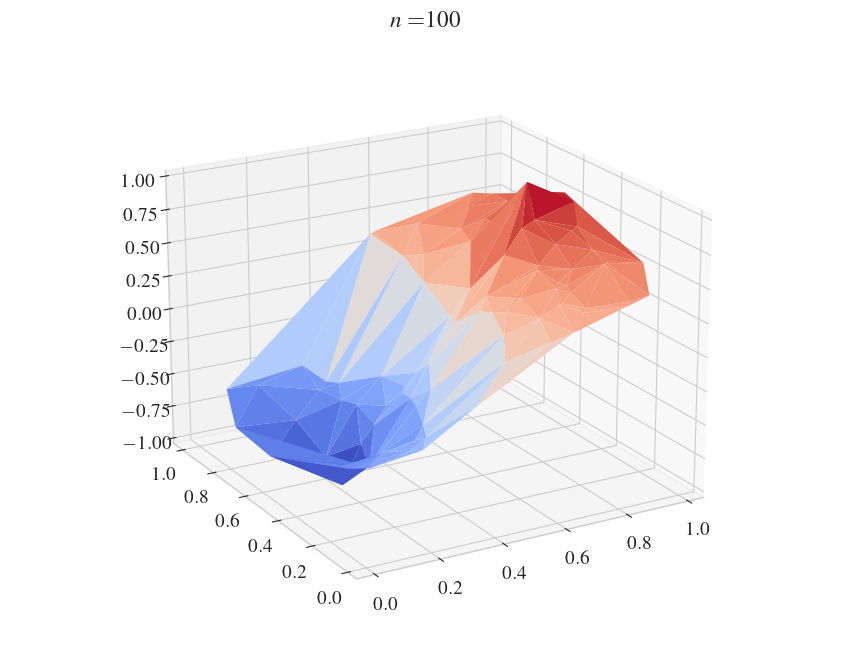
\includegraphics[width=.28\textwidth, trim={3.1cm 1cm 3.5cm 0cm},clip]{code/SSL/2Dex_100-p=inf.png}%
\hfill%
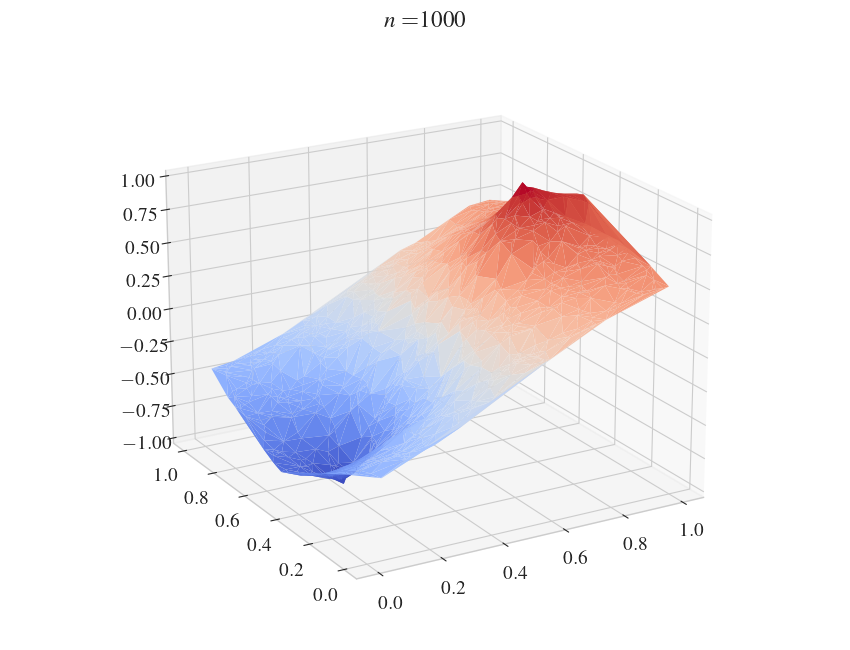
\includegraphics[width=.28\textwidth,trim={3.1cm 1cm 3.5cm 0cm},clip]{code/SSL/2Dex_1000-p=inf.png}%
\hfill%
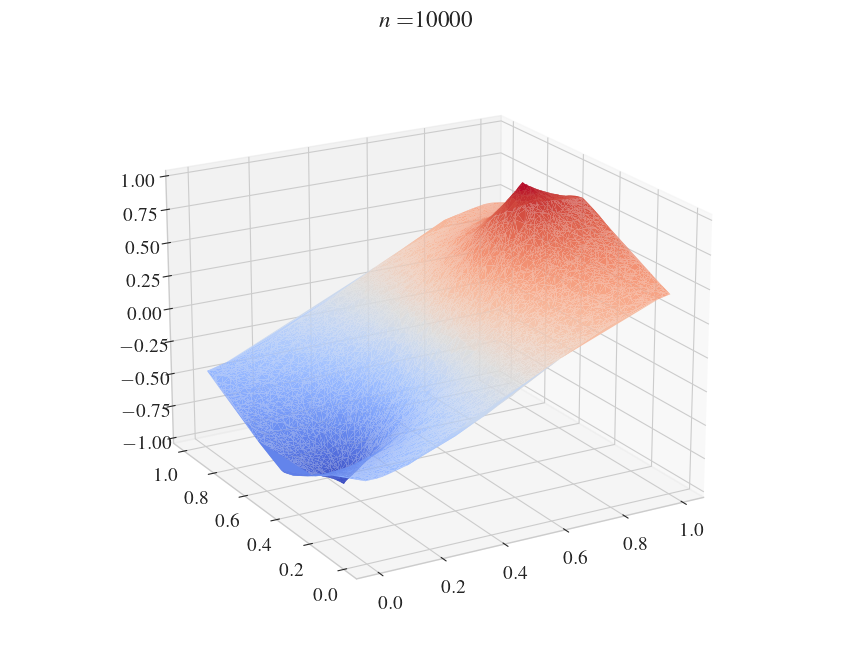
\includegraphics[width=.28\textwidth,trim={3.1cm 1cm 3.5cm 0cm},clip]{code/SSL/2Dex_10000-p=inf.png}%
%
\caption[Solution to the Laplacian Learning problem for different number of data points.]{Solution to the Laplacian Learning problem ($p=\infty$) for different number of data points $n\in\{100,1000,10000\}$. The setup is otherwise copied from \cref{ex:pLapBad}.}\label{fig:pinf}
\end{figure}
%
However, as already noticed in \cite{el2016asymptotic} being a pure $L^\infty$ problem, Lipschitz learning does not respect the density of data in any way. Namely, the method is exclusively distance based. This behavior is a drawback in many machine learning applications. However, by carefully rescaling the graph weights one obtains a data sensitive problem, see \cite{calder2019consistency} and \cref{sec:GConv}. 

The contributions presented in this chapter are all connected to the Lipschitz learning task. Namely, we are able to show consistency and convergence rates under very mild scaling assumptions.
%
%
%
%
%
%
%
\section{Lipschitz Extensions and the Infinity Laplacian: Continuum and Graph}\label{sec:LipExt}
%
Our main point of interest in this chapter is the Lipschitz learning task and its continuum limit. In this section we first motivate the continuum problem as considered in \cite{roith2022continuum, bungert2021uniform, bungert2022ratio}. We then given some details on the discrete problem.
%
%
\subsection{The Continuum Setting}\label{sec:LipExtCont}
%
%
We first recall, that for 
$u\in W^{1,\infty}(\domain)$ we have that
%
\begin{align*}
\lim_{p\to\infty} \pDir{}_{p,\rho}(u)^{1/p} = \esssup_{x\in\supp(\rho)} \abs{\nabla u(x)} =: \pDir{}_{\infty,\rho}(u),
\end{align*}
%
see \cite{jensen1993uniqueness}. Again, we see that that the weighting $\rho$ only enters via its support, therefore we do not explicitly consider it in the following and instead assume $\domain=\supp(\rho)$ and then only write $\pDir{}_{\infty}$. The functional $\pDir{}_\infty$ is weak$^*$-lower semi-continuous over $W^{1,\infty}(\domain)$, (see e.g. \cite[Thm. 2.6]{barron2001lower}). In the classical theory developed by Jensen in \cite{jensen1993uniqueness} one considers the following problem, which tries to \enquote{minimize the \emph{sup-norm} of the gradient} as described by Jensen.
%
\begin{problem}{Gradient Sup-Norm Problem}{prob:gradsup}
For an open domain $\domain\subset\R^d$ find a function $u\in W^{1,\infty}(\domain)$ such that
%
\begin{align*}
\norm{\nabla u}_\infty \leq \norm{\nabla v}_\infty \text{ for every } v, \text{s.t. } (u-v)\in W^{1,\infty}_0.
\end{align*}
\end{problem}
%
\noindent%
This problem can be seen as the limit problem for $p\to\infty$ of \cref{prob:VarForm}. Additionally imposing boundary conditions with $g:\partial\domain\to\R$, \cite{jensen1993uniqueness} then draws the connection to so-called \emph{Lipschitz extensions}, which are the driving concept in this section. We introduce a more general viewpoint---that does not require the notion of a gradient---later on, but first introduce the variational problem. 

\paragraph{The intrinsic metric and the Lipschitz constant.}

As noticed in \cite{jensen1993uniqueness} working with the Lipschitz constant and the sup-norm of the gradient requires a careful 
treatment of the distance measurement. Let $\tilde\domain$ be a set and let $d(\cdot,\cdot)$ be a semi-metric on $\tilde\Omega$, that is $d(\cdot,\cdot)$ fulfills 
the requirement of a metric up to triangle inequality. Then we define the Lipschitz constant of a function $u:V\to \R$ on a subset $V\subset \tilde\domain$ as
%
\begin{align*}
\Lip_d(u; V):= \sup_{x,y\in V, x\neq y} \frac{\abs{u(x) - u(y)}}{d(x,y)}.
\end{align*}
%
If $d(\cdot,\cdot)$ denotes the Euclidean distance we omit the subscript. i.e. $\Lip_d = \Lip$. Additionally, we can 
introduce the space of Lipschitz functions $\Lip_d(V)$ on $V$ via 
$u\in \Lip_d(V) \Leftrightarrow \Lip_d(u;V) <\infty$.
%
\begin{remark}{Lipschitz and Sobolev functions}{}
If $\domain\subset\R^d$ is sufficiently regular, e.g., it has Lipschitz boundary then we have that
%
\begin{align*}
\Lip(\domain) = W^{1,\infty}(\domain),
\end{align*}
%
where this identity is of course to be understood in the sense of equivalence classes in $\L^p$ spaces. We refer to \cite{evans2018measure} for a proof of this result.
\end{remark}
%
The above remark already relates Lipschitz with $W^{1,\infty}$ functions. Often however, we need a quantitative 
comparison between the Lipschitz constant and the sup-norm of the gradient of a function. Here, it is essential 
which distance measure is chosen for the Lipschitz constant. For an open domain $\domain\subset\R^d$ we have the inequality
%
\begin{align*}
\norm{\nabla u}_\infty \leq \sup_{x\neq y} \frac{\abs{u(x) - u(y)}}{\abs{x-y}}
\end{align*}
%
which can be proven via the definition of the gradient. For the reverse inquality, one has to respect the 
geometry of the domain, namely for $x,y\in\domain$ we have that
%
\begin{align}\label{eq:LipGrad}
\abs{u(x) - u(y)} \leq \norm{\nabla u}_\infty\ d_\domain(x,y)
\end{align}
%
see, e.g., \cite[Prop9.3, Rem. 7]{brezis2011functional}, where
%
\begin{align*}
d_\domain(x,y) = \inf \left\{
\int_0^1 \abs{\dot{\gamma}(t)} dt : \gamma\in C^1([0,1], \domain)\text{ with } \gamma(0)=x, \gamma(1) =y
\right\}
\end{align*}
%
denotes the \emph{geodesic distance} on $\domain$. If $\domain$ is convex, we have that $d_\domain(x,y) = \abs{x-y}$ for every 
$x,y\in \domain$ and therefore \cref{eq:LipGrad} yields $\Lip(u) = \norm{\nabla u}_\infty$. However, this situation changes for non-convex domains, see \cref{ex:tube}. Additionally it is often necessary to define 
a distance measure on the closure of $\domain\subset\R^d$. In order to have a geodesic on $\overline{\domain}$ one can simply consider $d_{\overline{\domain}}$, see e.g. \cite{bungert2021uniform}, which then yields the length space $(\overline{\domain}, d_{\overline{\domain}})$. In the classical theory developed in \cite{jensen1993uniqueness} one alternatively considers
%
\begin{align*}
\tilde{d}_{\overline{\domain}}(x,y) := \liminf_{(\tilde x,\tilde y)\to(x,y)} d_\domain(\tilde{x},\tilde{y}).
\end{align*}
%
The differences between these notions are demonstrated in the following example. Also note, that $\tilde{d}_{\overline{\domain}}$ is only a semi-metric on $\overline{\domain}$ since it is lacking a triangle inequality.
%
\begin{example}{}{ex:tube}
For $I = [-\pi, c]\cup [c, \pi]$ with $c=\pi/6$ we consider the domain
%
\begin{align*}
\bigcup_{\theta \in I} B_1\left((\cos(\theta),\sin(\theta)\right)
\end{align*}
%
which is visualized in \cref{fig:tube} and the points $x=(2\, c, 1), y= (2\, c, -1)$. The 
line segment between $x$ and $y$ contains the point $z=(2\, c, 0)$, however $z\notin \domain$. One can show that 
the geodesic has the length $d_\domain(x,y) = 4\, \cos(\pi/6) + \pi \approx 6.606$ which is the length of the dotted path 
in \cref{fig:tube}. However, we observe that 
%
\begin{align*}
\overline{\domain} = \bigcup_{\theta \in I } 
\overline{B_1\left((\cos(\theta),\sin(\theta)\right)}
\end{align*}
%
and in particular $z\in \overline{B_1\left((c,c)\right)}$, therefore $d_{\overline{\domain}}(x,y) = 2$.
\end{example}
%
\begin{figure}
\centering
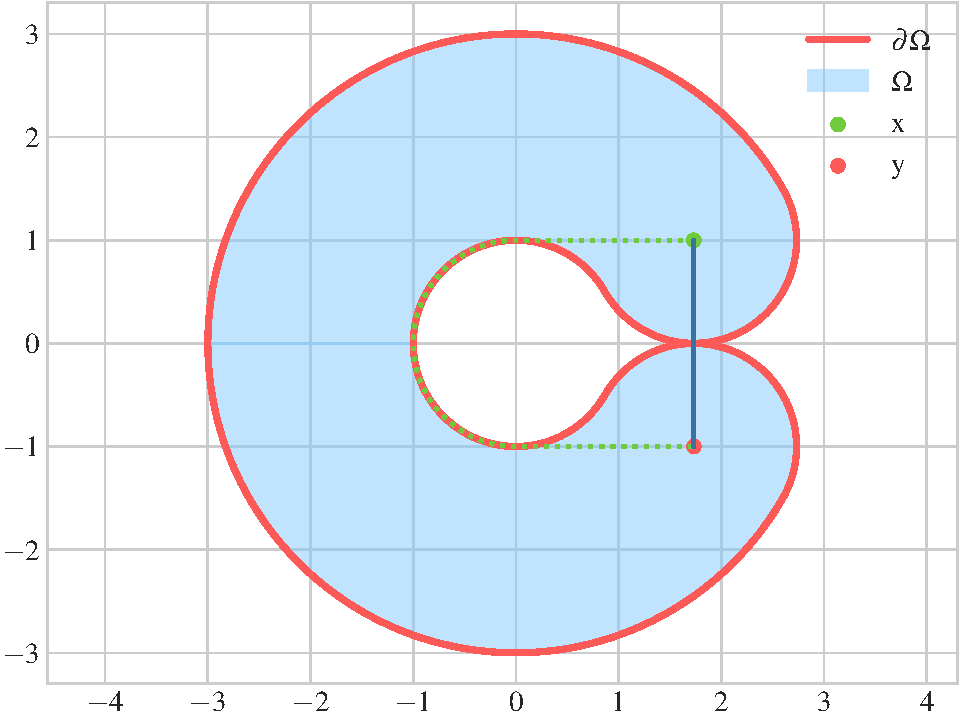
\includegraphics[width=.5\textwidth]{code/domains/tube.pdf}
\caption{The domain in \cref{ex:tube}.}\label{fig:tube}
\end{figure}
%
%
\paragraph{Solutions to the Gradient Sup-Norm Problem} Before generalizing the theory of Lipschitz extension to arbitrary metric spaces, we first note, that one can explicitly construct solutions of \cref{prob:gradsup}. Namely, for given $g\in\Lip(\partial\domain)$ the functions 
%
\begin{align}\label{eq:JenSol}
\begin{aligned}
\overline{g}(x) &:= \inf_{y\in\partial\domain} g(y) + 
\Lip_{\tilde{d}_{\overline{\domain}}}(g; \partial\domain)\cdot \tilde{d}_{\overline{\domain}}(x,y)\\
%
\underline{g}(x) &:= \sup_{y\in\partial\domain} g(y) - 
\Lip_{\tilde{d}_{\overline{\domain}}}(g; \partial\domain)\cdot \tilde{d}_{\overline{\domain}}(x,y)
\end{aligned}
\end{align}
%
are solutions to the gradient sup-norm problem that coincide with $g$ on $\partial\domain$, see \cite[Th. 1.8]{jensen1993uniqueness}.
%
\begin{remark}{}{}
The same concept of constructing solutions is applied in the following sections in a more abstract setting. 
These solutions are then called Whitney and McShane or respectively maximal and minimal extensions, see 
\cref{lem:ext}.
\end{remark}
%
One easily observes that there are cases where $\overline{g}\neq \underline{g}$ and therefore the problem does not admit a unique solution. A concrete example, to showcase this phenomena is given in \cite[p. 53]{jensen1993uniqueness}.
%
%
\paragraph{Lipschitz Extensions in Metric Spaces} The problem considered in the last section was motivated by a variational problem for $\pDir_\infty(u)=\norm{\nabla u}_\infty$. However, the theory of Lipschitz extensions provides a more general framework. Namely, here we do not assume that $\domain$ is a subset of 
$\R^d$ and rather consider a metric space $(\tilde{\domain},d)$ with $\domain\subset \tilde\domain$. 
%
\begin{remark}{}{}
For applications within this thesis we have that $\domain\subset\R^d$ is an open bounded domain and then consider 
$\tilde\domain:= \closure\domain$, i.e., the closure of $\domain$ within the topology induced by the Euclidean distance. 
In this abstract setting however, we use any metric space $\tilde\domain$ while still being close notation wise.
\end{remark}
%
%
%
\noindent%
A result originally due to Kierszbraun \cite{Kirszbraun1934} states that for two Hilbert spaces $\Inp, \Oup$, a subset $\conset\subset \Inp$ and a function $g:\conset\to \Oup$ there exists a function $u:\Inp\to \Oup$ such that 
%
\begin{align*}
u &= g \text{ on } \mathcal{O},\\
\Lip(u; \Inp) &= \Lip(g; \conset).
\end{align*}
%
Here, the metrics for the respective Lipschitz constants are induced by the inner products of the Hilbert spaces. We refer to \cite{Kirszbraun1934} for the original proof and to \cite[Th. 1.31]{Schwartz1969} for a proof of the version as stated above.
In this work we only consider the case $\Oup=\R$ which allows for more general assumption on the space $\Inp$. We now formulate the Lipschitz extension problem in our setting.
%
\begin{problem}{Lipschitz Extensions}{prob:Lipext}
Let $(\tilde{\domain},d)$ be a metric space and $\conset\subset \tilde{\domain}$ be a bounded subset. For a given Lipschitz function $g:\conset\to\R$ find a Lipschitz function $u:\tilde\domain\to \R$ such that
%
\begin{align*}
\Lip_d(u; \tilde\domain) = \Lip_d(g; \conset).
\end{align*}
%
A function $u:\tilde{\domain}\to\R$ with this property is called \emph{Lipschitz extension} of 
$g$ to $\tilde{\domain}$.
\end{problem}
%
\noindent%
In this setting one can explicitly construct solutions of the Lipschitz extension task. They are not unique, however one has an upper and a lower bound. In fact, conceptually these solutions 
are very similar to the functions in \cref{eq:JenSol} and even coincide, whenever the sup-norm of the gradient is given as the Lipschitz constant.
%
\begin{lemma}{}{lem:ext}
In the setting of \cref{prob:Lipext} we have that the 
%
\begin{itemize}
\item \textbf{Whitney (or maximal) extension:} $\Whit{g}(x) := \inf_{y\in \conset} g(y) + \Lip_d(g; \conset)\cdot d(x,y)$ and the
\item \textbf{McShane (or minimal) extension:} $\McS{g}(x) := \sup_{y\in \conset} g(y) - \Lip_d(g; \conset)\cdot d(x,y)$
\end{itemize}
%
defined for $x\in\tilde\domain$ are Lipschitz extensions of $g$ to $\tilde\domain$. Moreover, let $u:\tilde\domain\to\R$ be any Lipschitz extension of 
$g$, the we have that
%
\begin{align*}
\McS{g} \leq u \leq \Whit{g}.
\end{align*} 
\end{lemma}
%
\begin{proof}
We refer to \cite{whitney1992analytic} and \cite{mcshane1934extension} for the proofs of the respective result.
\end{proof}
%
\noindent%
As demonstrated in \cref{ex:maxprinc}, there are cases where $\Whit{g}\neq\McS{g}$ and 
therefore, Lipschitz extensions are not unique in general. Furthermore, \cite{aronsson2004tour} points out that the Whitney and McShane extension do not allow for a comparison principle, which can also be observed in \cref{ex:maxprinc}.
%
\begin{example}{}{ex:maxprinc}
Consider the set $\tilde\domain = [-1,1]$ and $\conset=\{-1,0,1\}$ with 
%
\begin{align*}
\color{apple}g_1\bc(x)&:= 0,\\
\color{grape}g_2\bc(x)&:= 1/2\ (x- \abs{x}),\\
\color{sky}g_3\bc(x)&:= -\color{grape}g_2\bc.
\end{align*}
%
Then we have that $\color{grape}g_2\bc\leq \color{apple}g_1\bc$ on $\conset$ but 
%
\begin{align*}
\color{grape}\Whit{g_2}\bc>\color{apple} \Whit{g_1}\bc \text{ in } (0,1),
\end{align*}
%
see \cref{fig:maxprinc} for a visualization. Analogously, we have that $\color{sky}g_3\bc\geq \color{apple}g_1\bc$ on $\conset$ but 
%
\begin{align*}
\color{sky}\McS{g_3}\bc<\color{apple} \McS{g_1}\bc \text{ in } (0,1).
\end{align*}
\end{example}
%
\begin{figure}
\centering
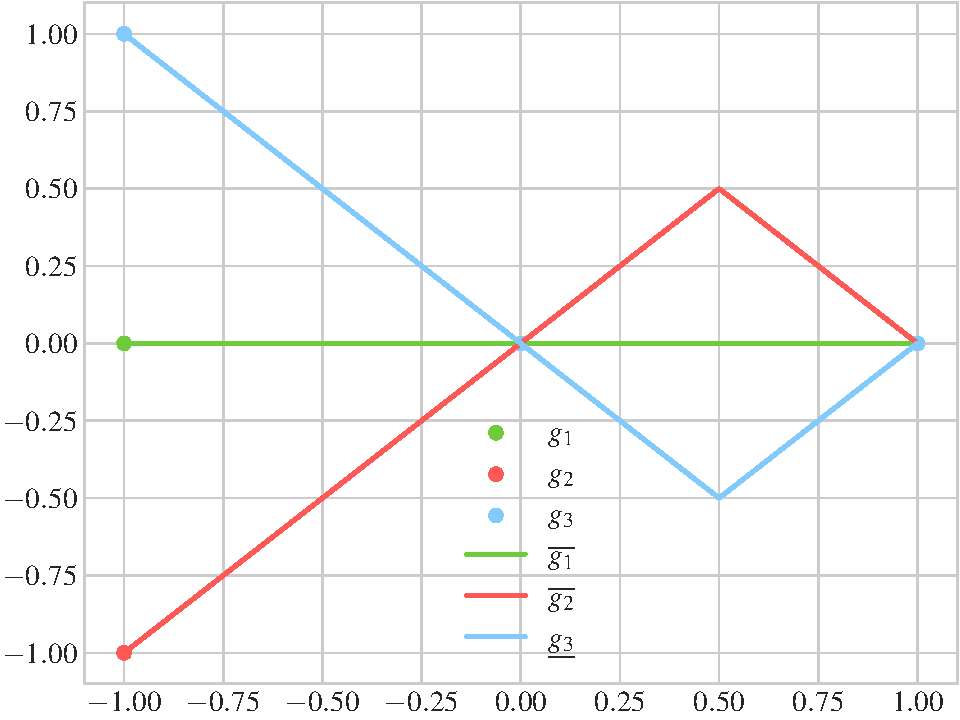
\includegraphics[width=.5\textwidth]{code/lipextcomp/comp.pdf}
\caption[Visualization for \cref{ex:maxprinc}.]{The maximal extension does not admit a comparison principle, as demonstrated in \cref{ex:maxprinc}.}\label{fig:maxprinc}
\end{figure}
%
%
\paragraph{Absolutely Minimizing Extension}\label{sec:AMLE}
%
Sending $p\to\infty$ in the variational formulation of the $p$-Laplace equation 
yields the Lipschitz extension task, which however does not admit for unique solutions. So the question arises, which property is lost in the limit case. For $p<\infty$ one has the local minimization property, as explained in \cref{sec:CSSL}. This lead Aronsson to introduce the concept of \emph{absolutely minimizing Lipschitz extension} in \cite{aronsson1967extension}, by additionally enforcing the minimizing property on every subset. A function $u\in W^{1,\infty}$ is called absolutely minimal, iff
%
\begin{align}\label{eq:absmin}
\esssup_{x\in V} \abs{\nabla u} \leq \esssup_{x\in V} \abs{\nabla v} \text{ for every open } V\subset \domain
\end{align}
%
and every function $v$ such that $(u-v)\in W^{1,\infty}_0$. In fact in \cite{aronsson1967extension} it is also shown, that 
$u_p\xrightarrow{p\to\infty} u_\infty$, which seems to validate the notion of absolute minimizers. In \cite{aronsson2004tour} it was shown, that one has an equivalent formulation involving the Lipschitz constant. For a given Lipschitz function $g:\overline{\domain}\to\R$ we have that $u_\infty$ with $(u_\infty-g)\in W^{1,\infty}_0(\domain)$ fulfills \cref{eq:absmin} iff
%
\begin{align*}
\Lip(u_\infty; V) \leq \Lip(v; V) \text{ for every } V\subset \domain
\end{align*}
%
and every function $v$ such that $(u-v)\in W^{1,\infty}_0(V)$, see \cite{aronsson1967extension}. In this thesis we work with a notion of absolute minimizers, which is equivalent to the above formulation for convex domains in $\R^d$. However, for our applications it is more convenient to formulate the problem for abstract length spaces.
%
\begin{problem}{AMLEs}{prob:amles}
Let $(\tilde{\domain}, d)$ be a length space, $\conset\subset\tilde{\domain}$ a closed subset and $g:\conset\to\R$ a Lipschitz function. Find an extension $u\in C(\tilde{\domain})$ such that $u=g$ on $\conset$ and
%
\begin{align}\label{eq:amlewg}
\Lip_d(u; \overline{V}) = \Lip_d(u, \partial V) \text{ for all open and connected sets } V\subset \tilde{\domain}\setminus \conset.
\end{align}
%
A function $u$ fulfilling this property is called absolutely minimizing Lipschitz extension of $g$.
\end{problem}
%
\begin{remark}{}{}
In our setting $\domain$ is an open subset of $\R^d$ and we then choose $\tilde{\domain} = \overline{\domain}$. Here, it is important to note that 
the topological notions like boundary and interior are to be understood relative to $\overline{\domain}$. A visualization of this concept can be found in \cref{fig:relb}.
\end{remark}
%
\begin{figure}
\begin{center}
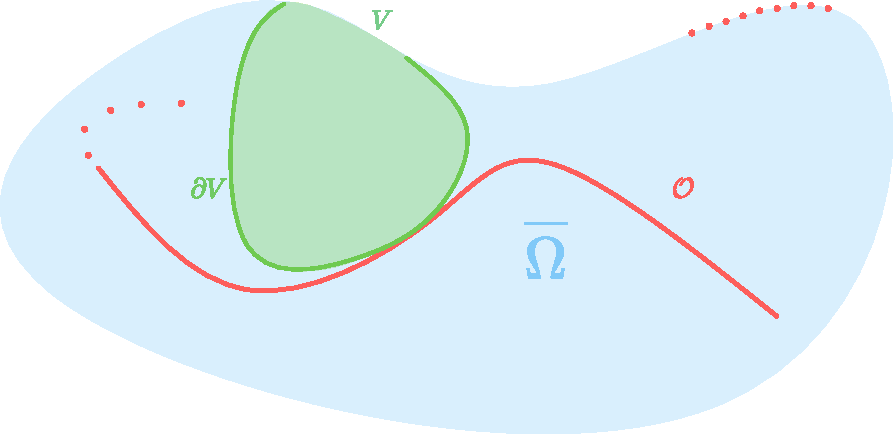
\includegraphics[width=.5\textwidth]{atelier/SSL/relboundary.pdf}
\end{center}
\caption[Visualization of the relative boundary.]{A set $V\subset\overline{\domain}$ can be relatively open w.r.t. the metric space $\overline{\domain}$ although, $V\cap\partial\domain \neq\emptyset$, where $\partial \domain$ is the boundary within the standard topology on $\R^d$. The relative boundary of $\partial_{\overline{\domain}} V$ does not include any parts of $\partial \domain$.}\label{fig:relb}
\end{figure}
%
%
\noindent%
Fulfilling \cref{eq:amlewg} also makes sense without enforcing boundary conditions on some set $\conset$. Typically, one just says $u$ is absolutely minimizing (AM) if it \cref{eq:amlewg} holds, see \cite{aronsson2004tour}. In the convex and Euclidean case, existence of solutions to \cref{prob:amles} follow directly from Aronssons proof that the limit $u_p\xrightarrow{p\to\infty} u_\infty$ fulfills \cref{eq:absmin}, see \cite{aronsson1967extension}. For general length spaces, it can be shown via an adapted Perron's method \cite{perron1923neue}, which we state in the following result from \cite{juutinen2002absolutely}.

\begin{theorem}{\cite[Th. 4.3]{juutinen2002absolutely}}{thm:examle}
Let $(\tilde\domain, d)$ be a separable length space, and suppose $g: \conset\to\R$ is Lipschitz. Then there exists an absolutely minimizing Lipschitz extension $u$ of $g$ to $\tilde\domain$, i.e. $u$ solves \cref{prob:amles}.
\end{theorem}
%
\noindent%
We address the question of existence and uniqueness of solutions to \cref{prob:amles} in the following paragraphs.
%
%
\paragraph{The Infinity Laplacian} In the Euclidean case one can derive an operator equation by considering the limit of the $p$-Laplacian operator. This yields the $\infty$-Laplacian which is defined as
%
\begin{align*}
\Delta_\infty u = \langle \nabla u, D^2 u\, \nabla u\rangle = 
\sum_{i,j} \partial_{x_i} u\, \partial_{x_j} u\, \partial_{x_i,x_j} u
\end{align*}
%
for functions of class $C^2$. This operator had one of its first appearances in \cite{aronsson1968partial}, but we refer to \cite{lindqvist2017notes} for a detailed overview of the topic. The brief exposition here, also follows \cite{lindqvist2017notes} to some extent. Intuitively the $\infty$-Laplace operator gives the second derivative of $u$ into the direction of its gradient. The associated infinity Laplace equation takes the following form.
%
\begin{problem}{}{prob:inflap}
Let $\domain\subset\R^d$ be an open and bounded domain and $g\in W^{1,\infty}$, then the task is to find $u$ such that
%
\begin{align*}
\Delta_\infty u &= 0\quad\text{ in }\domain,\\
u &= g\quad \text{ on }\partial\domain.
\end{align*}
\end{problem}
%
\noindent%
At first glance, the definition of the $\infty$-Laplacian only makes sense for for functions of class $C^2$. However, as shown in \cite{yu2006remark, aronsson1968partial} if $u\in C^2(\domain)$ fulfills $\Delta_\infty u = 0$ in $\domain$, then either $\nabla u \neq 0$ in the whole domain or it is constant. However on can easily construct boundary values $g$ that are not constant but force the solution $u$ to have critical points inside of the domain, see e.g. \cite{lindqvist2016notes}. Therefore, one requires a different concept, where one typically considers \emph{viscosity solutions}. For the $\infty$-Laplacian this strategy was first employed in \cite{bhattacharya1989limits}, where the term \emph{viscosity} is motivated by similar concepts for the Burgers' equation \cite{burgers1948mathematical}. First we consider subsolutions, where we take any $\phi\in C^2(\domain)$ that touches $u$ from above at any $x\in\domain$, i.e.
%
\begin{align}\label{eq:visc}
u < \phi \text{ in } \domain\setminus\{x\}\qquad\text{ and } u(x) = \phi(x).
\end{align}
%
Since we $\phi$ is $C^2$ we can shift the application of $\Delta_\infty$ onto this functions and then say $u$ is a subsolution if for any $\phi$ fulfilling \cref{eq:visc} we have
%
\begin{align*}
- \Delta_\infty \phi(x) \leq 0.
\end{align*}
%
Note, that the $\infty$-Laplacian is only evaluated at the touching point $x\in\domain$. Analogously, we say $u$ is a supersolution if for any $\phi$ touching from below we have $- \Delta_\infty \phi(x) \geq 0$. If $u$ is both a sub- and a supersolution, we say it is a solution in the viscosity sense. 
%
\begin{remark}{}{}
The concept of viscosity solutions can similarly be applied to the $p$-Laplacian or even a more general class of differential operators, see \cite{lindqvist2017notes}. We also note, that one has the consistency result, that if $u\in C^2$ is a viscosity solution, we also have that $\Delta_\infty u = 0$ in the classical sense. 
\end{remark}
%
%
\noindent%
Solving the $\infty$-Laplace equation in the viscosity sense is in fact equivalent to being absolutely minimizing, which we state in the following theorem taken from \cite{aronsson2004tour}
%
\begin{theorem}{\cite[Theorem 4.13]{aronsson2004tour}}{th:compprinc}
A function $u\in C(\cl\domain)$ fulfills $\Delta_\infty u=0$ in $\domain$ in the viscosity sense iff it is an absolutely minimizing function on $\domain$.
\end{theorem}
%
%
\noindent
In \cref{prob:inflap} we only consider the case where boundary values are given on $\partial\domain$. However, for our application we would rather have a Dirichlet condition on the set $\conset\subset\cl\domain$, since it often does not make sense to prescribe boundary values on $\partial\domain$. Therefore, we assume Neumann boundary conditions on this boundary and then consider the problem
%
\begin{align}\label{eq:inflapneumann}
\begin{aligned}
\Delta_\infty u = 0 &\text{ in }\domain\setminus\conset\\
\frac{\partial u}{\partial \nu} = 0 &\text{ on }\partial\domain\setminus\conset\\
u = g &\text{ on }\conset.
\end{aligned}
\end{align}
%
In the case that $\domain$ is smooth and convex, from \cite[Lem. 3.1]{armstrong2011infinity} we have that $u\in C(\cl\domain)$ is an AMLE of $g:\conset\to\R$ to $\cl\domain$ iff it fulfills \cref{eq:inflapneumann}.\par

We can now also address the question of uniqueness, where we state the following famous result of Jensen \cite{jensen1993uniqueness}.
%
\begin{theorem}{\cite{jensen1993uniqueness}}{th:jens} 
Let $u,v\in C(\cl\domain)$ be two viscosity solutions of the $\infty$-Laplacian, then we have
%
\begin{align*}
\max_{\cl\domain} (u - v) = \max_{\partial\domain} (u - v).
\end{align*}
\end{theorem}
%
%
\noindent%
Originally proven by Jensen in \cite{jensen1993uniqueness}, there exists a very simple proof by Amstrong and Smart \cite{armstrong2010easy} employing the \emph{comparison with cones} which we detail in the following paragraph.
%
%
%
\paragraph{Comparison with Cones} As shown in \cite{aronsson2004tour} the concept of absolutely minimizing extensions is equivalent to so-called \emph{comparison with cones}. For some metric $d(\cdot,\cdot)$ a cone function is defined as
%
\begin{align*}
x\mapsto a\, d(x,z) + c
\end{align*}
%
where $z\in\domain$ denotes the origin or cone tip, $a\geq 0$ its opening angle and $c\in\R$ some offset. The property we consider in the following basically asks, if a function $u$ is smaller than a cone on the boundary of some set $V$ not including the tip $z$, then it should be smaller also in the interior of the domain. This means for any $a\geq 0,c\in\R$ and $z\notin V$ we have the implication
%
\begin{align*}
\left[u \leq a\, d(\cdot,z) + c \text{ on }\partial V\right]
\quad \Rightarrow\quad
\left[u \leq a\, d(\cdot,z) + c \text{ in } V\right].
\end{align*}
%
%
One can omit the explicit use of the offset $c\in\R$ and equivalently consider the property
%
\begin{align}\label{eq:conecont}
\max_{\partial V}\left(u - a\, d(\cdot,z)\right) = \max_{V}\left(u - a\, d(\cdot,z)\right)
\end{align}
%
which is reminiscent of the comparison principle in \cref{th:compprinc}. In the Euclidean case cone functions are infinity harmonic away from their cone tip, since they are constant in the direction of their gradient. We make the explicit computation below
%
\begin{align*}
\partial_{x_i} \abs{x-z} &= \frac{x_i - z_i}{\abs{x-z}}\\
\partial_{x_i x_j}\abs{x-z} &= -\frac{(x_i - z_i)\, (x_j - z_j)}{\abs{x-z}^3}\text{ for } i\neq j,\\
\partial_{x_i}^2\abs{x-z} &= \frac{1}{\abs{x-z}^3} \sum_{j\neq i} (x_j - z_j)^2,\\
\Rightarrow
\Delta_\infty \abs{x-z} &= 
%
\sum_{i} \frac{(x_i - z_i)^2}{\abs{x-z}^5} \, \sum_{j\neq i} (x_j - z_j)^2\\
&\quad-\sum_{i\neq j}\frac{(x_i - z_i)^2\, (x_j - z_j)^2}{\abs{x-z}^5} = 0.
\end{align*}
%
%
In the Euclidean case as in \cite{aronsson2004tour} one says a function fulfills \emph{comparison with cones} from above, if it fulfills \cref{eq:conecont} in $\domain$ for every subset $V\subset\subset\domain$, every $a\geq 0$ and $z\in\R^n\setminus V$. We say $u$ fulfills \emph{comparison with cones} from below if $-u$ fulfills comparison from above. If it fulfills both comparisons from above and below, we say it fulfills comparison with cones. Here, \cite[Prop. 2.1]{aronsson2004tour} shows the following equivalence to being absolutely minimizing, which however mainly focuses on the Euclidean case. Our setting slightly deviates from the Euclidean one, where in \cite{bungert2021uniform} we consider the following notion.
%
\begin{definition}{\cite[Def. 4.1]{bungert2021uniform}}{def:comparison_distance_functions}
We shall say that a upper semicontinuous function $u\in USC(\closure \domain)$ satisfies CDF from above in $\cl\domain\setminus\constr$, if  for each relatively open and connected subset $V \subset \cl\domain\setminus\constr$, any \revision{$x_0\in \closure\domain\setminus V$} and $a\geq 0$ we have
\[\max_{\closure V}(u - a\,d_{\cl\domain}(x_0,\cdot)) = \max_{\revision{\relpartial V}}(u - a\,d_{\cl\domain}(x_0,\cdot)).\]
Similarly, we say  $u\in LSC(\closure\domain)$ satisfies CDF from below in $\cl\domain\setminus\constr$, if for each relatively open and connected subset \revision{$V\subset \cl\domain\setminus\constr$}, any \revision{$x_0\in \closure\domain\setminus V$} and $a\geq 0$ we have
\[\min_{\closure V}(u + a\,d_{\cl\domain}(x_0,\cdot)) = \min_{\revision{\relpartial V}}(u + a\,d_{\cl\domain}(x_0,\cdot)).\]
We say $u\in C(\closure\domain)$ satisfies CDF if it satisfies CDF from above and below.
\end{definition}
%
\noindent%
This definition is a special case of the notion in \cite{juutinen2006equivalence}. Therein, the authors also show the equivalence to the absolutely minimizing property, which we state in the following.
%
%
\begin{theorem}{\cite[Prop. 4.1]{juutinen2006equivalence}}{}
A function $u\in C(\cl\domain)$ is absolutely minimizing iff it fulfills comparison with cones in $\domain$.
\end{theorem}
%
\noindent%
Therefore, we can rewrite \cref{prob:amles} employing the comparison with cones condition. Our metric space is given as $(\cl\domain, d_{\cl\domain})$, where $\domain\subset\R^n$ is some open set in the Euclidean sense, therefore we have a separable length space, where \cref{thm:examle} yields existence of solutions for \cref{prob:amles}. Concerning uniqueness, we refer to \cite{peres2009tug} which were the first to prove uniqueness in the length space setting. For a more general result we refer to \cite{naor2012absolutely}. In our work we obtain uniqueness by a careful adaption of the proof in \cite{armstrong2010easy}, which we state here for completeness.
%
\begin{proposition}{\cite[Prop. 4.11]{bungert2021uniform}}{}
Consider the metric space $(\cl\domain, d_{\cl\domain})$, then \cref{prob:amles} has at most one solution.
\end{proposition}
%
%
\subsection{Graph Lipschitz Extensions}\label{sec:GLipExt}
%
We now consider the limit $p\to\infty$ of \cref{prob:vargraph} in the graph case. Analogously to \cref{sec:LipExtCont} we derive
%
\begin{align*}
\lim_{p\to\infty} \left(\GE^{w_n}_p(\vec u)\right)^{1/p}= \max_{x,y\in\domain_n} w_n(x,y) \abs{\vec u(y) - \vec u(x)}=:\GE^{w_n}_\infty(\vec u)
\end{align*}
%
which extends the graph $p$-Dirichlet energy to the case $p=\infty$. Again we notice structural similarities to 
the continuum version $\pDir_\infty$. 
%
\begin{remark}{}{}
Informally speaking the functional $\GE^{w_n}_\infty$ combines elements of a gradient and a Lipschitz constant. Assuming that $w_n(x,y)$ relates to $1/\abs{x-y}$ we see that the finite difference approximation
resembles a Lipschitz constant. However, in the limit $n\to\infty$ the weighting $w_n(x,y)$ has a localizing property which fits the interpretation of a gradient better.
\end{remark}
%
\noindent%
This functional now yields the graph Lipschitz extension problem.
%
\begin{problem}{Graph Energy Minimization}{prob:lipgraph}
Given a weighted graph $(\domain_n, w_n)$ and a labeling function $\vec g:\conset_n\to\R$, for $\conset_n\subset\domain_n$ we consider 
the problem
%
\begin{align*}
\min_{\vec u:\domain_n\to\R} \GE_\infty^{w_n}(\vec u) \text{ subject to } \vec u(x) = \vec g(x) \text{ for all } x\in\conset_n.
\end{align*}
\end{problem}
%
\noindent%
Since the weighting function $w_n:\domain_n\times\domain_n\to\R^+_0$ does not induce a metric, \cref{prob:lipgraph} does not directly fit the framework of the abstract Lipschitz Extension in \cref{prob:Lipext}. However, we can consider paths in $(\domain_n, w_n)$, connecting arbitrary $x,y\in\domain_n$ i.e. $\gamma\in\domain_n^{\times k}, x=\gamma_1,\ldots, \gamma_k = y$ such that 
%
\begin{align*}
w_n(\gamma_i, \gamma_{i+1}) &> 0\quad\text{for all } i=1,\ldots, k-1,
\end{align*}
%
for which we define the length as
%
\begin{align*}
\abs{\gamma} = \sum_{i=1}^{k-1} w_n(\gamma_i, \gamma_{i+1})^{-1}.
\end{align*}
%
This yields the metric space $(\domain_n, d_{w_n})$, where $d_{w_n}:\domain_n\times\domain_n\to\R$ is defined as
%
\begin{align}\label{eq:graphdist}
d_{w_n}(x,y) := \min \left\{ \abs{\gamma}: \gamma \text{ is a path in } 
(\domain_n, w_n)\text{ from } x \text{ to } y\right\}.
\end{align}
%
\begin{remark}{}{}
We note that it is important to only consider non-negative weights, otherwise any loop with a negative \enquote{length} would decrease the 
length of the whole path arbitrarily. However, restricting ourselves to non-negative weights we can easily see, that the minimum in \cref{eq:graphdist} is indeed attained.
\end{remark}
%
\noindent%
With this definition we can consider the Lipschitz extension task of $g:\conset_n\to\R$ to $\domain_n$ within the metric space $(\domain_n,d_{w_n})$, i.e. within the setting of \cref{prob:Lipext}. Therefore the question arises, whether the minimization problem in \cref{prob:lipgraph} is equivalent to the metric Lipschitz extension problem for which we have the following lemma.
%
%
\begin{lemma}{}{}
For a graph $(\domain_n, w_n)$ with non-negative weights and a function $\vec u:\domain_n\to\R$ we have that 
\begin{align*}
\GE_\infty^{w_n}(\vec u) = \Lip_{d_{w_n}}(\vec u).
\end{align*}
%
Furthermore, for $\conset_n\subset\domain_n$ and a function $\vec g:\conset_n\to\R$ and we have that
%
\begin{align*}
\vec g = \vec u \text{ on } \conset_n\Rightarrow
\Lip_{d_{w_n}}(\vec g;\conset_n) \leq \Lip_{d_{w_n}}(\vec u).
\end{align*}
\end{lemma}
%
%
\begin{proof}
\textbf{Step 1:} We show that $\Lip_{d_{w_n}}(\vec u) \leq \GE_\infty^{w_n}(\vec u)$.\\
%
We can choose a path $\gamma\in\domain_n^{\times k}$ such that
%
\begin{align*}
\Lip_{d_{w_n}}(\vec u) &= \frac{\vec u(\gamma_1) - \vec u(\gamma_k)}{\abs{\gamma}}.
\end{align*}
%
The path $\gamma$ allows to compare vertices $\gamma_1, \gamma_k\in\domain_n$ that aren't necessarily neighbors in the graph. However, each consecutive vertices in the path are neighbors in the graph and therefore we have
%
\begin{align}\label{eq:gebound}
w_n(\gamma_i, \gamma_{i+1}) \abs{\vec u(\gamma_{i+1}) - \vec u(\gamma_i)}
&\leq \GE^{w_n}_\infty(\vec u)\quad \text{ for all } i=1,\ldots, k-1.
\end{align} 
%
We now employ an elementary result for numbers $a_i\in\R^+_0, b_i\in\R^+, i=1,\ldots m\in\N$, namely
%
\begin{align}\label{eq:basicineq}
\left[
a_i\cdot b_i \leq c\in\R \quad\text{ for }
i=1,\ldots, m
\right]
%
\quad\Rightarrow\quad
%
\frac{\sum_{i=1}^{m}a_i}{\sum_{i=1}^{m} b_i^{-1}} \leq c
\end{align}
%
which can be seen as follows
%
\begin{align*}
a_i\cdot b_i &\leq c\quad\text{ for } i=1,\ldots, m,\\
\Rightarrow
a_i &\leq b_i^{-1}\cdot c \quad\text{ for } i=1,\ldots, m,\\
\Rightarrow\sum_{i=1}^{m} a_i &\leq \left(\sum_{i=1}^m b_i^{-1}\right)\cdot c,\\
%
\Rightarrow\frac{\sum_{i=1}^{m} a_i}{\sum_{i=1}^{m} b_i^{-1}} &\leq c.
\end{align*}
%
This then yields 
%
\begin{align*}
\frac{\abs{\vec u(\gamma_1) - \vec u(\gamma_k)}}{\abs{\gamma}}\leq
\frac{\sum_{i=1}^{k-1} \abs{\vec u(\gamma_i) - \vec u(\gamma_{i+1})}}{\abs{\gamma}} = 
\frac{\sum_{i=1}^{k-1} \abs{\vec u(\gamma_i) - \vec u(\gamma_{i+1})}}{\sum_{i=1}^{k-1} w_n(\gamma_i, \gamma_{i+1})^{-1}}
%
\leq
\GE^{w_n}_\infty(\vec u) 
\end{align*}
%
where in the last inequality we employed \cref{eq:basicineq} together with \cref{eq:gebound}.\\
%
\noindent%
\textbf{Step 2:} We show that $\Lip_{d_{w_n}}(\vec u) \geq\GE_\infty^{w_n}(\vec u)$.\\
%
Let $x,y\in \domain_n$, then we know that $d_w(x,y) \leq w_n(x,y)^{-1}$ and therefore
%
\begin{align*}
\abs{\vec u(x) - \vec u(y)} w_n(x,y)\leq 
\frac{\abs{\vec u(x) - \vec u(y)}}{d_w(x,y)} \leq 
\max_{\bar{x}, \bar{y}\in\domain_n}  
\frac{\abs{\vec u(\bar x) - \vec u(\bar y)}}{d_w(\bar x,\bar y)} = \Lip_{d_{w_n}}(\vec u).
\end{align*}
%
Since this holds for arbitrary $x,y\in\domain_n$ we have that
%
\begin{align*}
\GE^{w_n}_\infty(\vec u) = \max_{x,y\in\domain_n} \abs{\vec u(x) - \vec u(y)} w_n(x,y)
\leq
\Lip_{d_{w_n}}(\vec u).
\end{align*}\\
\noindent%
\textbf{Step 3:} We show that $\Lip_{d_{w_n}}(\vec g;\conset_n) \leq \Lip_{d_{w_n}}(\vec u)$.\\
%
If $\vec g = \vec u$ on $\conset$ this simply follows since the maximum for the Lipschitz constant of $\vec u$ is taken over a larger set. Indeed,

\begin{align*}
\Lip_{d_{w_n}}(\vec u) &= 
\max_{x,y\in\domain_n} \frac{\abs{\vec u(x) - \vec u(y)}}{d_w(x,y)}
\geq 
\max_{x,y\in\conset_n} \frac{\abs{\vec u(x) - \vec u(y)}}{d_w(x,y)}
=
\max_{x,y\in\conset_n} \frac{\abs{\vec g(x) - \vec g(y)}}{d_w(x,y)}\\
&=
\Lip_{d_{w_n}}(\vec u; \conset_n).
\end{align*}
\end{proof}
%
%
%
\noindent%
This lemma shows that the abstract Lipschitz extension task considered on the metric space $(\domain_n, d_{w_n})$ and the Graph $\infty$-Dirichlet minimization task are indeed equivalent. Therefore, we also have the Whitney and McShane extensions
%
\begin{align*}
\Whit{\vec g}(x) &= \inf_{y\in\conset_n} \vec g (y) + d_{w_n}(x,y)\\
\McS{\vec g}(x) &= \sup_{y\in\conset_n} \vec g (y) - d_{w_n}(x,y)
\end{align*}
%
as solutions on the graph. Analogously, the problem does not admit for unique solutions.
%
%
%
\paragraph{Absolutely Minimizing Graph Extensions}
%
Similarly to \cref{sec:AMLE} we can now consider absolutely minimizing extensions. However, the problem in 
\cref{prob:amles} uses a notion of a boundary and it is not directly clear how to infer this concept to the discrete set $\domain_n$. Therefore, we define the following what we mean by \enquote{boundary} on a graph.
%
\begin{definition}{}{}
Let $(\domain_n, w_n)$ be a weight graph and let $V\subset\domain_n$ be a subset, then we define
%
\begin{itemize}
\item the \textbf{exterior} boundary as $\partialext :=\{x\in \domain_n\setminus V: w_n(x,y) > 0 \text{ for some } y\in V\}$,
\item the \textbf{interior} boundary as $\partialint :=\{x\in V: w_n(x,y) > 0 \text{ for some } y\in \domain_n\setminus V\}$.
\end{itemize}
%
The closure of $V$ is then defined as $\extcl{V} := V\cup \partialext$ and the interior as 
$\stackrel{\circ}{V}^{\text{int}}:= V\setminus \partialint V$.
\end{definition}
%
%
\noindent%
We note that it is not possible to define a topology on $\domain_n$ that would yield the above notions. Namely, the only admissible topology in our case would be the discrete topology, i.e., $2^{\domain_n}$. However, in this topology the only closed sets are $\emptyset$ and $\domain_n$ which is not useful for the applications in the following. Using the Kuratowski closure axioms \cite{kuratowski1922operation} we remark the following.
%
\begin{lemma}{}{}
The exterior closure on a weighted graph $(\domain_n, w_n)$ is a preclosure or Čech closure.
\end{lemma}
%
\begin{proof}
Here, we use the notion of a preclosure in \cite{vcech1966topological}.
We first see that $\overline{\emptyset}^{\text{ext}}=\emptyset$ and that $V\subset \overline{V}^{\text{ext}}$ for every subset $V\subset\domain_n$, i.e. the above defined closure preserves the empty set and is extensive. Furthermore, for two sets $V_1,V_2\subset \domain_n$ we have that
%
\begin{gather*} 
x\in \partialext (V_1\cup V_2)\\
\Leftrightarrow\left[x\notin V_1\cup V_2\right]\wedge \left[\exists y\in V_1\cup V_2: w_n(x,y) \right]\neq 0\\
\Leftrightarrow 
\left[x\notin V_1\cup V_2\right]\wedge
\bigg(\left[\exists y\in V_1: w_n(x,y) \neq 0 \right]\vee
\left[\exists y\in V_2: w_n(x,y) \neq 0 \right]\bigg)\\
\Leftrightarrow \left[x\in \partialext V_1\setminus V_2\right]\vee
\left[x\in  \partialext V_2 \setminus V_1 \right]\\
\Leftrightarrow x\in (\partialext V_1 \cup \partialext V_2)\setminus (V_1\cup V_2).
\end{gather*}
%
We have shown that $\partialext (V_1\cup V_2)=(\partialext V_1 \cup \partialext V_2)\setminus (V_1\cup V_2)$. Therefore, we have that
%
\begin{align*}
\extcl{V_1\cup V_2} &= 
V_1\cup V_2 \cup \partialext (V_1\cup V_2)\\
&= V_1\cup V_2 \cup ((\partialext V_1 \cup \partialext V_2)\setminus (V_1\cup V_2))\\
&= V_1\cup \partialext V_1 \cup V_2 \cup \partialext V_2\\
&= \extcl{V_1}\cup\extcl{V_2}.
\end{align*}
%
This shows that the closure preserves binary unions and therefore we have shown, that it is indeed a Čech closure.
\end{proof}
%
%
%
\noindent%
The missing property, that inhibits the closure to induce a topology is the so-called idempotence. Namely, there are sets $V\subset \domain_n$ such that
%
\begin{align*}
\overline{V}^{\text{ext}} \neq \extcl{\extcl{V}}.
\end{align*}
%
\begin{figure}
\centering
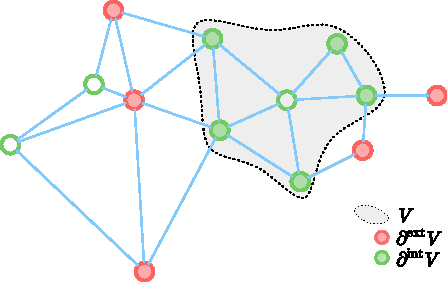
\includegraphics{atelier/SSL/boundary.pdf}
\caption{Visualization of exterior and interior boundary on a graph.}\label{fig:graphb}
\end{figure}
%
\noindent%
In the example visualized in \cref{fig:graphb} we see that $\overline{\overline{V}^{\text{ext}}}^{\text{ext}}=\domain_n\neq \overline{V}^{\text{ext}}$. Since the closure we employ here does not induce a topology, we have a slightly modified notion of absolutely minimizers.
%
\begin{problem}{Graph AMLEs}{prob:GAMLE}
Given a connected weighted graph $(\domain_n, w_n)$, $\conset_n\subset\domain_n$ and a function $\vec g:\conset_n\to\R$ find a function $\vec u:\domain_n\to\R$ such that
%
\begin{align*}
\Lip_{d_{w_n}}(\vec u; \extcl{V}) &= \Lip_{d_{w_n}}(\vec u; \partialext V)
\text{ for all connected } V\subset \domain_n\setminus\conset_n,\\
\vec u &= \vec g\text{ on } \conset_n.
\end{align*}
\end{problem}
%
\noindent%
This notion of absolute minimizers is employed in \cite{bungert2021uniform, bungert2022ratio}.  We see, that graph AMLEs are indeed special solutions of the basic Lipschitz extension problem on the graph, by choosing $V=\domain_n\setminus\conset_n$ in the above problem.
%
%
%
\paragraph{Comparison with Graph Distance functions}
%
Analogously to the continuum case \cref{sec:LipExtCont} we can also consider comparison with distance functions, but now on graphs. The main ingredients here, are the graph distance function $d_{w_n}$ and the notion of closure on a graph as developed in the last section.
%
%
\begin{definition}{}{}
For a weighted graph $(\domain_n,w_n)$ we say a function $\vec u:\domain_n\to\R$ fulfills comparison with distance function from above (CDFA) on a subset $U\subset \domain_n$ if for every $V\subset U$ we have
%
\begin{align}\label{eq:CDFA}\tag{CDFA}
\max_{\extcl{V}} \left(u - a\ d_{w_n}(\cdot, z)\right)=
\max_{\partialext V} \left(u - a\ d_{w_n}(\cdot, z)\right)
\end{align}
%
for every $z\in \domain_n\setminus V$ and every $a\geq 0$. We say that $\vec u$ fulfills comparison with distance function from below (CDFB) on a subset $U\subset \domain_n$ if for every $V\subset U$ we have
%
\begin{align}\label{eq:CDFB}\tag{CDFB}
\min_{\extcl{V}} \left(u + a\ d_{w_n}(\cdot, z)\right)=
\min_{\partialext V} \left(u + a\ d_{w_n}(\cdot, z)\right)
\end{align}
%
for every $z\in \domain_n\setminus V$ and every $a\geq 0$.
\end{definition}
%
%
\noindent%
Analogously to the continuum case, we say that a function fulfills comparison with distance functions, if it fulfills both, \labelcref{eq:CDFA} and \labelcref{eq:CDFB}. 
%
%Existence of such functions is established later, we are first interested in the question of uniqueness. Since the notion of graph boundaries is not directly compatible with the usual definitions on metric spaces, we prove it separately. Here, we adapt arguments from [smart] and [LeGruyer]. To do so we first consider the operators
%%
%\def\eps{\varepsilon}
%\begin{align*}
%\vec S^\eps \vec u (x) := \max_{y\in\domain_n: d_{w_n}(x,y)\leq \eps} \vec u(y) \quad
%\vec S_\eps \vec u (x) := \min_{y\in\domain_n: d_{w_n}(x,y)\leq \eps} \vec u(y)
%\end{align*}
%%
%and proof the following lemma, which is the analogue of 
%
%
\paragraph{The Graph $\infty$-Laplacian}
%
We can also obtain the limit of the Graph $p$-Laplace operator via the following formal calculation,
%
\begin{align*}
\Delta^{w_n}_p \vec u(x) &= 0\\
\Leftrightarrow \sum_{y\in\domain_n} w_n(x,y)^{p} \abs{\vec u(y) - \vec u(x)}^{p-2} (\vec u(y) - \vec u(x)) &= 0\\
%
\Leftrightarrow 
\sum_{y: \vec u(x)\leq \vec u(y)} w_n(x,y)^{p}(\vec u(y)-\vec u(x))^{p-1}
&= \sum_{y: \vec u(x)> \vec u(y)} w_n(x,y)^{p}(\vec u(x)-\vec u(y))^{p-1}.
%\\
%\Leftrightarrow
%\left(\sum_{y: \vec u(x)\leq \vec u(y)} w_n(x,y)^{p}(\vec u(y)-\vec u(x))^{p-1}\right)^{1/p}
%&=\\
%\left(\sum_{y: \vec u(x)> \vec u(y)} w_n(x,y)^{p}(\vec u(x)-\vec u(y))^{p-1}\right)^{1/p}
\end{align*}
%
Taking the terms on the left and right hand side to the power of $1/p$ and then formally sending $p\to\infty$ then yields
%
\begin{align*}
\max_{y: \vec u(x)\leq \vec u(y)} w_n(x,y)(\vec u(y)-\vec u(x)) &= 
\max_{y: \vec u(x) > \vec u(y)} w_n(x,y)(\vec u(x)-\vec u(y))\\
%
\Leftrightarrow \max_{y\in\domain_n} w_n(x,y)(\vec u(y)-\vec u(x)) &= 
-\min_{y\in\domain_n} w_n(x,y)(\vec u(y)-\vec u(x)).
\end{align*}
%
%
This calculation motivates the definition of the graph infinity Laplacian
%
\begin{align*}
\Delta_\infty^{w_n} \vec u(x) := \max_{y\in\domain_n} w_n(x,y)(\vec u(y)-\vec u(x)) +
\min_{y\in\domain_n} w_n(x,y)(\vec u(y)-\vec u(x)),
\end{align*}
%
which then allows to formulate the associated problem as an  extension of \cref{prob:graphLaplace}.

\begin{problem}{Graph $\infty$-Laplacian}{prob:graphinfLaplace}
Given a weighted graph $(\domain_n, w_n)$ and a labeling function $\vec g:\conset_n\to\R$ with $\conset_n\subset\domain_n$, find 
a function $\vec u:\domain_n\to\R$ such that
%
\begin{align*}
\Delta_\infty^{w_n} \vec u &= 0, \text{ in } \domain_n\setminus \conset_n,\\
\vec u &= \vec g \text{ on } \conset_n.
\end{align*}
\end{problem}
%
%
\noindent%
To establish existence of solutions of the problem above one can employ the Perron method \cite{perron1923neue}. Alternatively, one can establish the equivalence to so-called lex-minimizers and the show existence as in \cite[Th. 3.3]{kyng2015algorithms}. Uniqueness is a consequence of the following theorem from \cite{calder2019consistency}, which is similar to uniqueness lemma of Jensen \cref{th:jens}.
%
\begin{theorem}{\cite[Th. 3.1]{calder2019consistency}}{}
Let $(\domain_n,w_n)$ be a graph connected to the the boundary $\conset_n\subset\domain_n$ and consider $\vec u,\vec v:\domain_n\to\R$ such that
%
\begin{align*}
\Delta^{w_n}_\infty \vec u \leq 0 \leq \Delta^{w_n}_\infty \vec v
\quad\text{ in } \domain_n\setminus\conset_n.
\end{align*}
%
Then we know that
%
\begin{align*}
\max_{\domain_n} (\vec u - \vec v) = \max_{\conset_n} (\vec u - \vec v)
\end{align*}
\end{theorem}
%
%
\paragraph{Relations Between the Graph Lipschitz Extensions} We now establish the connection between the different notions of Lipschitz extensions on the graph. Compared to the continuum case we do not establish the full equivalences but only the necessary implications required for the convergence proofs in \cite{bungert2021uniform}. Namely, in \cite{bungert2021uniform} we show that if $\vec u$ solves the graph $\infty$-Laplace, then it is an graph AMLE and fulfills comparison with graph distance functions. 
%
%
\begin{lemma}{\cite[Th. 3.2, Prop. 3.8]{bungert2021uniform}}{}
Let $(\domain_n,w_n)$ be a weighted connected graph and $\vec g:\conset_n\to\R$ be a given function for $\conset_n\subset\domain_n$. Furthermore, let $\vec u:\domain_n\to\R$ be graph infinity harmonic on $\domain_n\setminus\conset_n$ with boundary conditions given by $\vec g$, i.e., $\vec u$ solves \cref{prob:graphinfLaplace} then we have that
%
\begin{itemize}
\item $\vec u$ is an graph AMLE, i.e., $\vec u$ solves \cref{prob:GAMLE},
\item $\vec u$ fulfills comparison with cones.
\end{itemize}
\end{lemma}
%
%
\begin{proof}
Both of the statements are proven in \cite{bungert2021uniform}. Let $\vec u$ be such that 
%
\begin{align*}
\Delta^{w_n}_\infty \vec u &= 0\text{ in }\domain_n \setminus \conset_n\\
\vec u &= \vec g \text{ on } \conset_n.
\end{align*}
%
From \cite[Prop. 3.8]{bungert2021uniform} we have that $\vec u$ is an graph AMLE. Furthermore, form \cite[Th. 3.2]{bungert2021uniform} we have that $\vec u$ fulfills comparison with cones. In fact, \cite[Th. 3.2]{bungert2021uniform}, shows a more refined statement, namely that
%
\begin{align*}
-\Delta^{w_n}_\infty \vec u &\leq 0 \Rightarrow \vec u \text{ fulfills \labelcref{eq:CDFA}},\\
-\Delta^{w_n}_\infty \vec u &\geq 0 \Rightarrow \vec u \text{ fulfills \labelcref{eq:CDFB}}.
\end{align*}
%
\end{proof}
%
%
%
%
\section{Gamma Convergence: \cite{roith2022continuum}}\label{sec:GConv}
We now present the main results of \cite{roith2022continuum}. This works considers the limit of the basic Lipschitz extension from the graph \cref{prob:lipgraph} to the continuum case \cref{prob:Lipext}. As detailed in the previous sections both of these problems do not admit for unique solutions, however it still meaningful to study the convergence in the infinite data limit. We first start by specifying the setting and recalling the concept of $\Gamma$-convergence and then state the main results.
%
%
\paragraph{Main Contributions in \cite{roith2022continuum}} We first prove $\Gamma$-convergence of the functionals $\GE^{w_n}_\infty$ to their continuum counterpart $\pDir_\infty$. This result can be seen as the extension of the results in \cite{GarcSlep15, slepcev2019analysis} to the case $p=\infty$. Here, we employ a different type of metric as we detail in the following. Furthermore, we identify the optimal graph scaling which in this case is derived in a deterministic manner. The key difference to \cite{GarcSlep15, slepcev2019analysis} is that we can work with any point-clouds and not only i.i.d. points. The inherent reason is that $L^\infty$ problems only consider mass in a qualitative not in a quantitative way. We then establish a compactness result, that allows us to infer convergence of minimizers. Finally, we apply this theory to the ground state problem.

Parts of this work was motivated by the findings in TR's master thesis \cite{roith2022msc}. The convergence result in the latter, was however not fully established and therefore \cite{roith2022continuum} constitutes a non-trivial expansion and also correction. We want to highlight two major differences:
%
\begin{itemize}
\item The domain $\domain$ in \cite{roith2022msc} was assumed to be convex. This restriction was omitted in \cite{roith2022continuum} by identifying a class of locally convex domains, that prevent internal sharp corners.
\item We are able to work with asymptotic boundary conditions, i.e., the boundary conditions for each graph problem do need to be the same as in the continuum. They only need to approximate them in some sense. 
\end{itemize} 
%
%
%
%
\subsection{Setting and Preliminaries}
%
Here, we detail the concrete setting of \cite{roith2022continuum} and provide some background on the employed notions.
%
%
\paragraph{$\Gamma$-Convergence} Originally, the concept of $\Gamma$-convergence dates back to De Giorgi \cite{de1975tipo} as a type of variational convergence. We refer to \cite{Brad02, dal2012introduction} for a detailed overview on this notion and related topics. While $\Gamma$-convergence was successfully employed in a pure continuum setting for a longer time (see e.g. \cite{modica1977esempio}), it was more recently used to prove convergence form a discrete to a continuum functional \cite{chambolle2010continuous, braides2012quantitative, van2012gamma}. 
%
%
%
\begin{definition}{\cite{de1975tipo}: $\Gamma$-convergence}{}
Let $X$ be a metric space and let $F_n:X\rightarrow [-\infty,\infty]$ be a sequence of 
functionals. We say that $F_n$ $\Gamma$-converges to the functional 
$F:X\rightarrow [-\infty,\infty]$ if
\begin{enumerate}[label=(\roman*)]
	\item \textbf{(liminf inequality)} for every sequence $(x)_{n\in\N}\subset X$ converging to 
	$x\in X$ we have that
	\begin{align*}
		\liminf_{n\rightarrow\infty} F_n(x_n) \geq F(x);
	\end{align*}
	\item\textbf{(limsup inequality)} for every $x\in X$ there exists a sequence 
	$(x)_{n\in\N}\subset X$ converging to $x$ and 
	\begin{align*}
		\limsup_{n\rightarrow\infty} F_n(x_n)\leq F(x).
	\end{align*}
\end{enumerate}
\end{definition}
%
\noindent%
The most relevant reference for \cite{roith2022continuum} was the disruptive work presented by Garc\'ia Trillos and Slep\v{c}ev in \cite{GarcSlep15}, which is also commented on in \cref{sec:GSSL}. Among other important ideas and notions, we want to highlight two ingredients that directly influenced \cite{roith2022continuum}:
%
\begin{itemize}
\item $\Gamma$-convergence on a common metric space, that allows to compare graph functions with continuum functions.
\item The proof strategy of first considering the discrete to non-local convergence and then non-local to continuum.
\end{itemize}
%
%
Employing $\Gamma$-convergence the authors in \cite{slepcev2019analysis} were able to prove convergence of minimizers of the graph $p$-Dirichlet problem. Here, one can employ the convenient result that $\Gamma$-convergence implies converrgence of minimizers.
%
\begin{lemma}{\cite[Thm. 1.21]{Brad02} Convergence of Minimizers}{lem:ConvMin}
	Let $X$ be a metric space and $F_n:X\rightarrow [0,\infty]$ a sequence of 
	functionals $\Gamma$-converging to $F\rightarrow X:[0,\infty]$ which is not 
	identically $+\infty$. 
	If there exists a relatively compact sequence $(x_n)_{n\in\N}$ such that 
	\begin{align*}
		\lim_{n\rightarrow\infty} \left(F_n(x_n) - \inf_{x\in X} F_n(x)\right) = 0, 
	\end{align*}
	then we have that 
	\begin{align*}
		\lim_{n\rightarrow\infty} \inf_{x\in X} F_n(x) = \min_{x\in X} F(x)
	\end{align*}
	and any cluster point of $(x_n)_{n\in\N}$ is a minimizer of $F$.
\end{lemma}
%
%
\paragraph{The Kernel and the Graph Scale}
%
\begin{wrapfigure}[11]{r}{.5\textwidth}%
\tikzfading[name=fade out, 
inner color=transparent!0,
outer color=transparent!60]
\hspace*{2em}%
\vspace{-2em}%

\begin{tikzpicture}[scale=1.]%
\draw[fill=sky!10, draw = none, thick, dashed] plot [smooth cycle] coordinates {(-1,.1)(-0.2,5.5)(4,4.9)(4.5,3)(6,1)(4,-0.5)(2,-1)} node at (1.8,1.7) {};
%
\node (F) at (3.5,1.5) {};
\fill[apple!20,path fading = fade out] (F) circle (57pt);
%
\begin{scope}[every node/.style={circle,very thick,sky,draw,inner sep=2pt}]
	\node (A) at (0.7,1.9) {};
	\node (B) at (1.8,1.3) {};	
	\node[grape] (C) at (2.,5.2) {};
	\node[grape] (D) at (-0.7,2.5) {};
	\node[] (F) at (F) {};
	\node[grape] (G) at (-0.2,1.5) {} ;
	\node[grape] (E) at (0.2,3.8) {};
	\node (H) at (2.8,4) {};
	\node (I) at (2.5,3.) {};
\end{scope}

\draw[->,>=Latex,apple, thick] (F) -- 
+(-135:57pt) node[midway,below,sloped]{\small\nc$\sim \gscale_n$};

\node (Omega) at (0,5) {$\domain$};
\node (Omegan) at (3.5,4.2) {$\domain_n$};
\node (On) at ($(E)+(0.5,0.5)$) {$\conset_n$};

% boundary
\begin{scope}
	\clip (-0.5,-1.2) rectangle (3,6);
	\draw[fill=none, draw = grape, very thick, dashed] plot [smooth cycle] coordinates {(-1,.1)(-0.2,5.5)(4,4.9)(4.5,3)(6,1)(4,-0.5)(2,-1)} node at (2.2,5.7) {$\conset$};
\end{scope}
\draw[grape,very thick,dashed] plot [smooth] coordinates {(-0.5,-0.44)(-.7,.2)(0,3.5)(1.5,2.5)(2,3.0)};
%
\begin{scope}[every path/.style={sky}]
	\path [-] (A) edge (B);
	\path [-] (A) edge (E);
	\path [-] (A) edge (D);
	\path [-] (A) edge (G);
	\path [-] (D) edge (G);
	\path [-] (C) edge (H);
	\path [-] (D) edge (E);
	\path [-] (B) edge (F);
	\path [-] (I) edge (F);
	\path [-] (I) edge (B);
	\path [-] (I) edge (H);
\end{scope}
%
\node[circle,very thick,ponk,draw, fill, inner sep=2pt] (J) at (0.5,-0.5) {};
\path[draw=ponk, dotted, very thick] [-] (B) edge node[midway,below, sloped] {\small$\gres_n$} (J) ;
\end{tikzpicture}%
%
\end{wrapfigure}%

%
%
In \cref{sec:GSSL} we comment on the relevance of the kernel and graph scaling $\gscale_n$ for continuum limits. We first state the concrete assumptions we make in \cite{roith2022continuum} on the kernel $\eta:\R_0^+\to\R_0^+$, namely we require

\begin{enumerate}[label=(K\upshape\arabic*)]
	\item\label{en:K1} $\eta$ is positive and continuous at $0$,
	\item\label{en:K2} $\eta$ is non-increasing,
	\item\label{en:K4} $\supp(\eta) \subset [0,\etaradius_\eta]$ for some $\etaradius_\eta>0$.
\end{enumerate}
%
As seen in \cite{GarcSlep15, slepcev2019analysis} and \cref{eq:kernelconst} we also need to consider the constant $\sigma_\eta$ which in our case is given by
%
\begin{align*}
\sigma_\eta = \esssup_{t\in \R^+} \eta(t)\, t =
\lim_{p\to\infty} \left(\int_{\R^+} \eta(t)^p\, t^{d+p} dt\right)^{1/p}.
\end{align*}
%
%
A main difference to the results for $p<\infty$ is that we can work with point clouds $\domain_n$, that do not necessarily need be constructed by an i.i.d. sampling process. However, this rises the question how we can ensure that $\domain_n\subset\cl\domain$ fills out the continuum domain $\cl\domain$ sufficiently fast. In \cite{roith2022continuum} we consider the maximum distance of any continuum point to its next vertex
%
\begin{align}\label{eq:resolution}
\sup_{x\in\cl\domain} \min_{y\in\domain_n} \abs{x-y},
\end{align}
%
as a measure of the distance between $\domain_n$ and $\cl\domain$. In fact, this is the Hausdorff distance (\cite{hausdorff1914}) between the two sets, since 
%
\begin{align*}
d_H(\domain_n, \cl\domain) = 
\max
\left\{
\sup_{x\in\cl\domain} \inf_{y\in\domain_n} \abs{x-y},  
\sup_{x\in\domain_n} \inf_{y\in\cl\domain} \abs{x-y}
\right\} = 
\sup_{x\in\domain} \min_{y\in\domain_n} \abs{x-y},
\end{align*}
%
where the second term vanishes since $\domain_n\subset\cl\domain$.
%

\begin{remark}{}{}
We remark on the historical correctness of the name \enquote{Hausdorff} distance, motivated by the review in \cite{birsan2006one}. This distance can actually be contributed to Pompeiu, who employed a similar notion in \cite{pompeiu1905continuite}, which also relates to concepts developed in Fréchet's Ph.D. thesis \cite{frechet1906quelques}. Hausdorff modified this distance into the presented form in \cite{hausdorff1914}.
\end{remark}
%
%
\noindent%
We also allow the constraint set $\conset_n$ to vary with each $n\in\N$, therfore we also measure the distance between $\conset_n$ and the continuum constraint set $\conset\subset\cl\domain$, via
%
\begin{align*}
d_H(\conset_n, \conset) = 
\max
\left\{
\sup_{x\in\conset} \inf_{y\in\conset_n} \abs{x-y},  
\max_{x\in\conset_n} \inf_{y\in\conset} \abs{x-y}
\right\}
\end{align*}
%
where the second term does not vanish, because in general $\conset_n\nsubseteq\conset$. We assume that we have a Lipschitz continuous function $g:\cl\domain\to\R$ such that for each $n$ the boundary conditions are given by the function $\vec g_n = g\rvert_{\conset_n}$. In total we then need to control the graph resolution 
%
\begin{align*}
\gres_n := \max\{d_H(\domain_n, \cl\domain), d_H(\conset_n, \conset)\}.
\end{align*}
%
This then allows us to formulating our scaling assumption, namely we require that the graph resolution tends to zero faster than the graph scaling
%
\begin{align}\label{eq:scaling}
\frac{\gres_n}{\gscale_n}\longrightarrow 0, \quad n \to \infty,
\end{align}
%
which has similarly employed in \cite{penrose1999strong,penrose1999strong2}. This is the weakest possible assumption that ensures connectivity of the graph in the limit $n\to\infty$. However, compared to \cref{eq:garcscaling} it is more of deterministic nature, since we do not assume anything on how $\domain_n$ is created. In case of a i.i.d. point cloud one can show that
%
\begin{align*}
\gres_n \sim \left(\frac{\log n}{n}\right)^{1/d}
\end{align*}
%
see \cite{penrose1999strong2}, which is the setting in \cite{GarcSlep15}.
%
%
\paragraph{Assumptions on the Domain} As we mention in the introduction, we do not need to restrict ourselves to convex domains. However, for our convergence results, it is important that the geodesic distance 
%
\begin{align*}
d_\domain(x,y)=\inf\left\lbrace
\mathrm{len}(\gamma): \gamma:[a,b]\rightarrow\domain 
\text{ is a curve with }
\gamma(a)=x, \gamma(b) = y
\right\rbrace,
\end{align*}
%
is converges to the Euclidean distance if $x$ goes to $y$. We formulate this in the following assumption
%
\begin{align}\label{eq:cond_domain}
\lim_{\delta\downarrow0}\sup
\left\lbrace
\frac{d_\domain(x,y)}{\abs{x-y}}\,:\,
x,y\in\domain,\,\abs{x-y}<\delta\right\rbrace \leq 1.
\end{align}
%
The inherent reason that we need no enforces this, is that edges in the graph are allowed to communicate via their direct Euclidean distance, even if this line does not lie in $\domain$. While it would be easier to also consider the geodesic distance on the graph, this is unrealistic in many applications since we do not have access to the concrete shape of $\domain$. Most importantly, \cref{eq:cond_domain} prohibits sharp internal corners in the domain, see \cref{fig:sharp}. Furthermore, note that we consider the geodesic distance $d_\domain$ on the open domain $\domain$, not on its closure. Therefore, we also exclude situations of a touching boundary as in \cref{fig:tube}. In \cite{roith2022continuum} we also provide examples of domains fulfilling this condition.
%
\begin{figure}
\centering%
\begin{tikzpicture}[scale=1.5]
\begin{scope}
	\clip(1.2,1.0) rectangle (4.5,5.5);
	\clip(1.0,1.0) circle (4.1cm);
	
	\begin{scope}
		%\path [scope fading=my fading,fit fading=false] (1,0) rectangle (8,8);
		\path[fill=sky!30, draw = none, path fading=south] plot coordinates {(0,0)(0,8)(4,8)(2,2)(6,4)(8,0)} node at (1.8,1.7) {};
	\end{scope}
	\begin{scope}[every node/.style={circle,thick,sky,draw, inner sep=6pt}]
		\node (X1) at (2.5,4.5) {};
		\node (X2) at (2.25,3.75) {};
		\node (X3) at (2.0,3.0) {};
		\node (Y1) at (4.2,2.8) {};
		\node (Y2) at (3.5,2.45) {};
		\node (Y3) at (2.8,2.1) {};
	\end{scope}
	\node[circle,fill,draw,grape,inner sep=0pt] (Z) at ($(X1) - 1.03*(1,3)$) {};
	%\node[circle,fill=faulnat,inner sep=0,text=sky] (J) at (1.5,5.2) {$x$};
	
	\begin{scope}[every path/.style={grape,dotted,thick}]
		\path (X1) edge (X2);
		\path (X2) edge (X3);
		\path (Y1) edge (Y2);
		\path (Y2) edge (Y3);
	\end{scope}
	%\path[draw=sky] [-] (B) edge (J2);
	\path[grape,thick] (X3) edge (Z);
	\path[grape,thick] (Y3) edge node[sloped,below=5pt,pos=0.5] {\small\nc$d_{\domain}$} (Z);
	\begin{scope}[every path/.style={sky,dotted, thick}]
		\path (X1) edge  node[sloped, above] {\small$|x_i-y_i|$} (Y1);
		\path (X2) edge (Y2);
		\path (X3) edge (Y3);
	\end{scope}
\end{scope}
\end{tikzpicture}
%
\caption[An example of a sharp internal corner, violating \cref{eq:cond_domain}.]{An example of a sharp internal corner, violating \cref{eq:cond_domain}. The geodesic distance between the pairs of points converging to the corner point is bigger than then Euclidean one by a constant factor.}\label{fig:sharp}
\end{figure}
%
%

%
\subsection{$\Gamma$-Convergence of the Discrete Functionals} In order to show convergence of discrete functionals defined on $\domain_n$ to continuum functions acting on $\overline\domain$, one needs to define a common metric space. Employing results form \cite{trillos2015rate} in \cite{GarcSlep15} the authors introduced the space $TL^p$
%
\begin{align*}
TL^p :=\left\{(\mu, u): \mu\in \mathcal{P}(\domain), u\in L^p(\mu)\right\}
\end{align*}
%
together with the transport distance
%
\begin{align*}
d_{TL^p}((\mu, u), (\nu, v)) = \inf_{\pi\in \Gamma(\mu,\nu)}
\left(\int_{\domain\times\domain} \abs{x-y}^p + \abs{u(x) - v(y)}^p d\pi(x,y)\right)^{1/p}
\end{align*}
%
where $\Gamma(\mu,\nu)$ is the set of coupling between $\mu$ and $\nu$. A sequence $(\mu_n, u_n)$ converges to $(\mu,u)$ in $TL^p$ iff there exists a sequence of transportation maps $T_n:\domain\to\domain$ with $T_n\#\mu = \mu_n$ and 
%
\begin{align*}
\int_{\domain} \abs{x- T_n(x)} d\mu(x)\rightarrow 0
\end{align*}
%
such that $u_n\circ T_n \xrightarrow{L^p} u$, \cite[Prop. 3.12]{GarcSlep15}. Therefore, the maps $T_n$ allow to employ standard convergence in $L^p$. In order to transfer this situation to $L^\infty$ one could try to employ a $\infty$-Wasserstein distance. However, as argued in \cite{roith2022msc} the strategy does not transfer directly, since convergence in $W^\infty$ does not metrize weak convergence of measures \cite[Thm. 5.10]{santambrogio2015optimal}. However, as seen in \cite{roith2022continuum} one can employ a more direct argument. For problems in $L^p$ the conservation of mass was important for the maps $T_n$ (i.e. $T_n\#\mu = \mu_n$) such that the integrals could be transformed. This condition is irrelevant in $L^\infty$, namely we have the following analogous transformation rule in $L^\infty$.
%
\begin{lemma}{\cite[Lem. 2]{roith2022continuum}}{lem:suptrafo}
For two probability measures $\mu,\nu \in \mathcal{P}(\overline{\domain})$, a measurable map 
$T:\domain\rightarrow\domain$ which fulfills
\begin{enumerate}[label=\upshape(\roman*)]
\item $\nu<<T\#\mu$,
\item $T\# \mu<<\nu$,
\end{enumerate}
and for a measurable function $u:\domain\rightarrow\R$ we have that
\begin{align*}
\nu\operatorname{-}\esssup_{x\in\domain} u(x) = \mu\operatorname{-}\esssup_{y\in\domain} u(T(y)).
\end{align*}
\end{lemma}
%
%
\noindent%
We want to compare the discrete measure $\mu_n = \frac{1}{n}\sum_{x\in\domain_n} \delta_x$ to the target measure $\mu$. In this setting a closest point projection $p_n:\domain\to\domain_n$
%
\begin{align*}
p_n(x) \in \argmin_{y\in\domain_n} \abs{x- y}
\end{align*}
%
fulfills the assumption of \cref{lem:suptrafo}. This allows us to extend the functional $\GE^{w_n}_\infty$ in \cref{prob:lipgraph} to $L^\infty$ via
%
\begin{align}\label{eq:lipextend}
\GE^{w_n}_\infty(u) = 
%
\begin{cases}
\GE^{w_n}_\infty(\vec u) &\text{ if } u=\vec u \circ p_n,\text{ for some } \vec u :\domain_n\to\R,\\
\infty &\text{ else },
\end{cases}
\end{align}
%
which was similarly done in \cite{GarcSlep15, slepcev2019analysis}. Additionally, we incorporate the constraint on $\conset_n$ in \cref{prob:lipgraph} via
%
\begin{align*}
\GE^{w_n, \text{cons}}_\infty (\vec u):=
\begin{cases}
\GE(\vec u)&\text{ if } \vec u = \vec g \text{ on } \conset_n,\\
\infty &\text{ else},
\end{cases}
\end{align*}
%
with the analogous extension to $L^\infty$ as in \cref{eq:lipextend}. We can now state the first main result of \cite{roith2022continuum} that provides the $\Gamma$-convergence of the graph functionals.
%
%
\begin{theorem}{Discrete to continuum $\Gamma$-convergence}{thm:DCGamma}
Let $\domain\subset\R^d$ be a domain satisfying~\labelcref{eq:cond_domain}, let the kernel fulfill \labelcref{en:K1}-\labelcref{en:K4}, then for any null sequence $(\gscale_n)_{n\in\N}\subset(0,\infty)$ which satisfies the scaling condition~\labelcref{eq:scaling}
we have
\begin{align}
\GE^{n,\mathrm{cons}}_\infty \GConv \sigma_{\eta}~\pDir^\mathrm{cons}.
\end{align}
\end{theorem}
%
\noindent%
The main proof strategy here is similar to the one in \cite{GarcSlep15, slepcev2019analysis}. Namely one defines the non-local functional
%
\begin{align*}
\pDir^{\gscale}_\infty(u) := \frac{1}{\gscale}~\esssup_{x,y\in\domain}
\left\{
\eta_{\gscale}(\abs{x-y})\abs{u(x) - u(y)}
\right\},\quad\gscale>0
\end{align*}
%
for which we show that for any sequence $\gscale_n\to 0$ we have
\begin{align*}
\pDir^{\gscale_n}_\infty\GConv \sigma_{\eta}~\pDir_\infty,
\end{align*}
%
see \cite[Thm. 4]{roith2022continuum}. For the liminf inequality of the discrete functionals, one has to take special care of points $x,y\in\domain_n$ where $\eta_{\gscale_n}(\abs{p_n(x) - p_n(y)})=0$. We want to bound $\GE^{w_n}_\infty$ from below by $\pDir_\infty^{\gscale_n}$ for which we have to permit significant communication of $x$ and $y$ whenever $p_n(x)$  and $p_n(y)$ do not communicate. This can be done, (temporarily assuming $\eta$ is constant on $[0,t]$) by introducing a smaller length scale $\tilde{\gscale}$ such that
%
\begin{enumerate}[label=(\roman*)]
\item\label{ga} $\abs{p_n(x) - p_n(y)} > t\gscale_n\Rightarrow \abs{p_n(x) - p_n(y)}/\gscale_n < \abs{x-y}/\tilde{\gscale}$,
\item\label{gb} $\lim_{n\to\infty} \tilde{\gscale}/\gscale=1$.
\end{enumerate}
%
As shown in \cite{roith2022continuum} the choice $\tilde\gscale= \gscale - 2 \gres/t$ fulfills \labelcref{ga}. So in order to fulfill 
\labelcref{gb} we obtain the scaling condition
%
\begin{align*}
\lim_{n\to\infty} \frac{\gres_n}{\gscale_n} = 0\Rightarrow \lim_{n\to\infty} \frac{\gscale_n - 2 \gres_n/t}{\gscale_n} = 1 - \frac{2}{t} \lim_{n\to\infty} \frac{\gres_n}{\gscale_n} = 1.
\end{align*}
%
This then allows to prove the liminf inequality since $\GE^{w_n}_\infty(u_n)\geq \frac{\tilde{\gscale}_n}{\gscale_n} \pDir^{\tilde{\gscale}_n}_\infty(u_n)$ holds. The limsup inequality can then be shown by choosing the constant sequence, with some additional care for the changing constraint set $\conset_n$.
%
%
\subsection{Convergence of Minimizers}
%
The convenient aspect of $\Gamma$-convergence is, that under additional compactness properties it directly shows convergence of minimizers, \cite[Thm. 8]{Brad02}. This yields the second main result in \cite{roith2022continuum}.
%
%
\begin{theorem}{\cite[Thm. 2]{roith2022continuum}}{thm:ConvMinLip}
Let $\domain\subset R^d$ be a domain satisfying~\labelcref{eq:cond_domain}, 
let the kernel fulfil \labelcref{en:K1}-\labelcref{en:K4}, 
and $(\gscale_n)_{n\in\N}\subset(0,\infty)$ be a null sequence which satisfies the scaling 
condition~\labelcref{eq:scaling}.
Then any sequence $(u)_{n\in\N}\subset L^{\infty}(\Omega)$ such that 
\begin{align*}
\lim_{n\rightarrow\infty}\left(\GE^{n,\mathrm{cons}}_\infty(u_n) - 
\inf_{u\in L^{\infty}(\domain)}\GE^{n,\mathrm{cons}}_\infty(u)\right) = 0
\end{align*}
is relatively compact in $L^{\infty}(\domain)$ and 
\begin{align*}
\lim_{n\rightarrow\infty} \GE^{n,\mathrm{cons}}_\infty(u_n) = 
\min_{u\in L^{\infty}(\domain)}\sigma_{\eta}~\pDir^{\mathrm{cons}}_\infty(u).
\end{align*}
Furthermore, every cluster point of $(u_n)_{n\in\N}$ is a minimizer of 
$\pDir_{\mathrm{cons}}$. 
\end{theorem}
%
%
\noindent%
In order to show the compactness in the above theorem one employs the following lemma.
%
%
\begin{lemma}{\cite[Lem. 4]{roith2022continuum}}{lem:compfirst}
Let $(\domain,\mu)$ be a finite measure space and $K\subset L^{\infty}(\domain;\mu)$ be a bounded set w.r.t. $\norm{\cdot}_{L^{\infty}(\domain;\mu)}$ such that 
for every $\varepsilon>0$ there exists a finite partition $\{V_i\}_{i=1}^n$ of $\domain$ into subsets $V_i$ with positive and finite measure such that
\begin{align}\label{eq:partinf}
\mu\operatorname{-}\esssup_{x,y\in V_i} \abs{u(x) - u(y)} < \varepsilon\ \forall u\in K, i=1,\ldots,n,
\end{align}
then $K$ is relatively compact. 
\end{lemma}
%
\begin{remark}{}{}
The proof of this statement employs ideas from \cite[Lem. IV.5.4]{dunford1988linear} and appeared similarly in TR's master thesis. However, therein the statement was slightly wrong, which was corrected in \cite{roith2022continuum}.
\end{remark}
%
\noindent%
This lemma is the used to show that if a sequence $u_n$ fulfills
\begin{align*}
\sup_{n\in\N}\GE^{w_n,\text{cons}}_\infty(u_n)<\infty
\end{align*}
%
then it is relatively compact.
%
\subsection{Application to Ground States}
%
The convergence results of the previous paragraphs can be applied to the ground states problem. Namely, for a $p$-homogeneous functional $\pDir$---i.e. $\pDir{}(cu) = \abs{c}^p \pDir{}(u)$ for $c\in\R$---we consider the following problem
%
\begin{align*}
\min\left\lbrace \pDir(u) \,:\, \inf_{v\in\argmin \pDir{}}\norm{u-v} = 1 \right\rbrace,
\end{align*}
%
as studied in \cite{bung20}. In our setting, if $g\equiv 0$ then the functionals $\GE^{w_n,\text{cons}}_\infty$ and $\pDir^{\text{cons}}_\infty$ are $1$-homogeneous. In \cite[Th. 5]{roith2022continuum} we first show that the up to a global sign unique ground state of $\pDir^{\text{cons}}_\infty$ is a multiple of the distance function
%
\begin{align*}
d_{\conset}(x)=
\inf_{y\in\conset}d_\domain(x,y).
\end{align*}
%
%
We then employ the $\Gamma$-convergence results to show the convergence of discrete ground states to the above continuum one.
%
\begin{theorem}{\cite[Thm. 6]{roith2022continuum}: Convergence of Ground States}{thm:cgvc_GS}
Under the conditions of \cite[Thm. 1]{roith2022continuum} let the sequence $(u_n)_{n\in\N}\subset L^{\infty}(\domain)$ fulfill
\begin{align*}
    \vec u_n \in \argmin\left\lbrace
    \GE^{w_n,\mathrm{cons}}_\infty(\vec u) \,:\,\vec u\in L^{\infty}(\domain),\, \norm{\vec u}_{L^{p}}=1 \right\rbrace.
\end{align*}
Then (up to a subsequence) $\vec u_n\to u$ in $L^{\infty}(\domain)$ where
\begin{align*}
    u \in \argmin\left\lbrace
    \pDir^{\mathrm{cons}}_\infty(u) \,:\,u\in L^{\infty}(\domain),\, \norm{u}_{L^{p}}=1 \right\rbrace
\end{align*}
and it holds
\begin{align}\label{eq:cvgc_eigenvalues}
    \lim_{n\to\infty}{\GE^{w_n,\mathrm{cons}}_\infty(\vec u_n)} = \sigma_\eta~\pDir^{\mathrm{cons}}_\infty(u).
\end{align}
\end{theorem}


%
\section{Uniform Convergence of AMLES: \cite{bungert2021uniform}}\label{sec:UnifConv}
%
%
In the previous section we consider the limit of the Lipschitz extension task. The major limitations of this work are:
%
\begin{itemize}
\item The considered problem does not admit for unique solutions. The $\Gamma$-convergence framework does not directly allow to select certain minimizers, e.g. AMLEs, and consider the respective limit to continuum AMLEs.
%
\item We can only show qualitative convergence results. It is not directly possible to prove quantitative statements and convergence rates.
\end{itemize}
%
These drawbacks are the main motivation for the work presented in this section. We first state the main contributions and then provide details below.
%
\paragraph{Main Contributions in \cite{bungert2021uniform}} We prove a quantitative convergence results for discrete AMLEs to their continuum counterpart. Convergence was already established in \cite{calder2019consistency}, however employing a more restrictive scaling assumption and only allowing for smooth kernels $\eta$, which was due to the viscosity techniques employed. By using the AMLE characterization of infinity harmonic functions, we are able to show convergence rates under the weakest scaling assumption and allowing for very general kernels. This is done via a using a comparison principle on a homogenized length scale. The key insight we obtain in this work, is that convergence rates for graph distance functions imply rates for AMLEs. Finally, we examine some numerical convergence rates.
%
%
%
\subsection{Setting}
%
Conceptually, the basic setting is very similar to the previous one in \cref{sec:GConv}. We highlight some minor differences in the paragraphs below.
%
%
\paragraph{Assumptions on the Kernel}
%
We employ \labelcref{en:K2,en:K4} from \cite{roith2022continuum} and set $t_\eta =1$ for simplicity. However we do not need to assume continuity in $0$, i.e. \labelcref{en:K1}. Instead we additionally require the following.
%
\begin{enumerate}[label=(K\upshape\arabic*)]
\setcounter{enumi}{3}
\item\label{ass:kernel} We assume that there exists $t_0\in(0,1]$, chosen as the largest number with this property with $\sigma_\eta=t_0\eta(t_0)$.
\end{enumerate}
%
Assuming \labelcref{en:K2,en:K4,ass:kernel} allows for the so-called singular weights
%
\begin{align*}
\eta(t)=\frac{1}{t^p}1_{[0,1]}(t)
\end{align*}
%
with $p\in(0,1]$. As noted in \cite{bungert2021uniform} the above assumption is not redundant, since for example the function
%
\begin{align*}
\eta(t) = \frac{1}{t^{\frac{1}{t-1}+2}}1_{[0,1]}(t),\quad t>0,
\end{align*}
%
violates \labelcref{ass:kernel}, while fulfilling \labelcref{en:K2,en:K4}.
%
%
\paragraph{Assumptions on the Domain} Again we take the concept from \cite{roith2022continuum}, where we assume asymptotic convexity. We alter the \cref{eq:cond_domain} slightly to be more quantitative. We assume that there exists a function $\phi:[0,\infty)\to[0,\infty)$ with $\lim_{h\downarrow 0}\frac{\phi(h)}{h} = 0$ and $r_\domain>0$ such that 
\begin{equation}\label{eq:geodesic_euclidean}
d_{\cl\domain}(x,y) \leq |x-y| + \phi(\abs{x-y}), \quad \text{for all }x,y\in\domain\st |x-y|\leq r_\domain.
\end{equation}
%
Furthermore, for $\gscale>0$ we define $\sigma_\phi(\gscale) = \sup_{0 < s \leq \gscale}\frac{\phi(s)}{s}$. Note that we now employ the geodesic distance $d_{\cl\domain}$, i.e. path can also lie on the boundary of $\domain$.
%
%
\paragraph{Assumptions on the Labeling Function} The assumption on the labeling for each sub-problem is weakened even further. Namely, we do not assume the labels for each discrete problem to be given by the continuum constraint $g:\conset\to\R$. Instead we require 

\begin{enumerate}[label=(C\arabic*)]
\item\label{ass:dataA} $\sup_{n\in\N}\Lip_n(\vec g_n;\conset_n)<\infty$ and $\Lip_\domain(g;\conset)<\infty$,
\item\label{ass:dataB} there exists $C>0$ such that for all $z\in\conset$ it holds that $\abs{\vec g_n(\pi_{\conset_n}(z))-g(z)}\leq C\gres_n$.
\end{enumerate}
%
%
This assumption on the labeling function, is also connected to the no-noise and infinite data limit, see e.g. \cite{hoffmann2020consistency}.
%
%
\subsection{Convergence Results}
%
%
In \cite{roith2022continuum} the proof strategy relied on $\Gamma$-convergence. In \cite{bungert2021uniform} we use the comparison with cones characterization of AMLEs together with comparison principles for the infinity Laplace operator. An important strategy is to consider the homogenized operator
%
\begin{align}\label{eq:homop}
\Delta_\infty^\nlscale u(x) = \frac{1}{\nlscale^2}\left(\inf_{y\in B_\nlscale(x)}(u(y)-u(x))
+
\sup_{y\in B_\nlscale(x)}(u(y)-u(x))\right)
\end{align}
%
%
on the length scale $\nlscale>0$ which is typically larger than the graph scale $\gscale$. The results in the following are non-asymptotic, for which also our scaling assumption reads as follows
%
\begin{align}\label{ass:scaling}
\begin{aligned}
\gscale &\leq {r_\domain,} \\
\frac{\gscale}{\nlscale} &< \frac{1}{2}, \\
\sigma_\phi(\gscale) + \frac{\res_n}{\gscale} 
&\leq
\frac{t_0}{4+2\sigma_\phi(\gscale)}
\left(1-2\frac{\gscale}{\nlscale}\right).
\end{aligned}
\end{align}
%
for some $n\in\N$. We detail the concrete appearance of the operator $\Delta^\tau_\infty$ in the following paragraphs and first state the main general result. We employ the notation $a\lesssim b$ which means that $a\leq C\,b$ for some constant $C>0$ depending only on $g$ and $\eta$, but not on $n, \gscale$ or $\gres$.
%
\begin{theorem}{\cite[Th. 2.2]{bungert2021uniform}}{thm:general_convergence_result}
Let $\nlscale>0$, let the kernel and data fulfill \labelcref{en:K2,en:K4,ass:kernel}, \labelcref{ass:dataA,ass:dataB} and let \labelcref{eq:geodesic_euclidean,ass:scaling} hold. Let $\vec u_n:\domain_n\to\R$ solve \cref{prob:GAMLE}, and $u:\closure\domain\to\R$ solve \cref{prob:amles}.
\begin{enumerate}
\item It holds 
\begin{align*}
    \sup_{\domain_n}\abs{u-\vec u_n} = \sup_{\closure\domain}\abs{u- u_n} \lesssim \nlscale +  \sqrt[3]{\frac{\res_n}{\gscale\nlscale} + \frac{\gscale}{\nlscale^2}+\frac{\phi(\gscale)}{\gscale\nlscale}}.
\end{align*}
\item If $\inf_{\cl\domain}\abs{\nabla u}>0$, then it even holds 
\begin{align*}
\sup_{\domain_n}\abs{u-\vec u_n} = \sup_{\closure\domain}\abs{u- u_n} \lesssim \nlscale +  {\frac{\res_n}{\gscale\nlscale} + \frac{\gscale}{\nlscale^2}+\frac{\phi(\gscale)}{\gscale\nlscale}}.
\end{align*}
%
Here, $u_n:\closure\domain\to\R$ denotes the piecewise constant extension of $\vec u_n$, as in \labelcref{eq:lipextend}.
\end{enumerate}
\end{theorem}
%
%
\noindent%
We observe that in the case where $\abs{\nabla u}$ is bounded away from zero the rate improves, which is due to a perturbation we briefly mention in the following. The parameter $\nlscale$ appears due to our proof strategy and does not have a concrete meaning for the final problem. An immediate consequence is that for an arbitrary $\nlscale>0$ we obtain
%
\begin{align*}
\sup_{\domain_n}\abs{u-\vec u_n} < \nlscale
\end{align*}
%
by sending $\gres_n,\gscale_n$ to zero as $n\to\infty$ employing the weakest scaling assumption $\gres_n\ll \gscale_n$. Since $\nlscale >0$ was arbitrary this already yields convergence of discrete AMLEs under the weakest scaling assumption \cite[Cor. 2.3]{bungert2021uniform}. In order to obtain the convergence rates involving only $\gres$ and $\gscale$ we can \enquote{optimize} over $\nlscale$. We first consider the small length scale regime, which in our case includes any graph scaling such that $\gscale\lesssim \gres_n^{5/9}$. In that case we can choose $\nlscale = ((\delta_n + \phi(\gscale))/\gscale)^{1/4}$ to obtain
%
%
\begin{align*}
\sup_{\domain_n}\abs{u-\vec u_n}
=
\sup_{\closure\domain}\abs{u-u_n} 
\lesssim\left(\frac{\res_n + \phi(\gscale)}{\gscale}\right)^\frac{1}{4}.
\end{align*}
%
%
If $\abs{\nabla u}$ is bounded away from zero this can be improved to 
%
\begin{align*}
\sup_{\domain_n}\abs{u-\vec u_n} 
=
\sup_{\closure\domain}\abs{u-u_n} 
\lesssim \left(\frac{\res_n + \phi(\gscale)}{\gscale}\right)^\frac{1}{2}.
\end{align*}
%
where we consider the regime $\gscale\lesssim\gres^{3/5}$. In the convex case, i.e. $\phi\equiv 0$ we therefore directly obtain the rates
%
\begin{align*}
\inf_{\cl\domain}\abs{\nabla u} = 0 &:
\left(\frac{\gres_n}{\gres_n^{5/9}}\right)^{\frac{1}{4}} = \gres_n^{\frac{1}{9}},\\
\inf_{\cl\domain}\abs{\nabla u} > 0 &:
\left(\frac{\gres_n}{\gres_n^{3/5}}\right)^{\frac{1}{2}} = \gres_n^{\frac{1}{5}},
\end{align*}
%
see \cite[Cor. 2.4]{bungert2021uniform}. In fact the convexity assumption is too strict, instead we just have to require that $\phi(\gscale)\lesssim \gscale^p$ for some power of $p\in\R^+$ that does not deteriorate the rate. This is done in \cite[Cor. 2.5, 2.6]{bungert2021uniform}, where also a better rate is obtained by allowing for larger length scales. In the following we sketch the main ingredients of the proof. While in the $\Gamma$-convergence case we employ the hierarchy
%
\begin{center}
\enquote{discrete $\to$ non-local $\to$ continuum}
\end{center} 
%
%
our scheme now has the form
%
\begin{center}
\enquote{discrete $\to$ homogenized non-local $\leftarrow$ continuum}.
\end{center}
%
We discuss the two directions below and then discuss how to \enquote{meet in the middle}.
%
\paragraph{Non-Local to Continuum}
%
In this paragraph we comment on how to relate continuum AMLEs to the homogenized operator in \cref{eq:homop}. Here, it is convenient to copy the following definitions from \cite{bungert2021uniform},
%
\begin{alignat}{2}
\label{eq:T-operators}
T^\nlscale u(x) &:= \sup_{\closure B_\domain(x,\nlscale)} u, 
\qquad
T_\nlscale u(x) &&:= \inf_{\closure B_\domain(x,\nlscale)} u,
\\
\label{eq:slopes}
S_\nlscale^+ u &:= \frac{1}{\nlscale}(T^\nlscale u - u),
\qquad
S_\nlscale^- u &&:= \frac{1}{\nlscale}(u-T_\nlscale u),
\end{alignat}
%
so that we can write $\Delta_\infty^\nlscale u = \frac{1}{\nlscale}\left(S^+_\nlscale u - S^-_\nlscale u\right)$. The astonishing property of this operator is the so-called \enquote{max-ball} lemma. If $u\in USC(\cl\domain)$ fulfills comparison with distance functions from above, then we have that the function $T^\nlscale u$ fulfills
%
\begin{align}\label{eq:maxballa}
-\Delta^\nlscale_\infty T^\nlscale u \leq 0, \quad\text{ in }
\domain_\conset^{2\nlscale},
\end{align}
%
analogously if $u\in LSC(\cl\domain)$ fulfills CDF form below we have
%
\begin{align}\label{eq:maxballb}
-\Delta^\nlscale_\infty T_\nlscale u \geq 0, \quad\text{ in }
\domain_\conset^{2\nlscale}.
\end{align}
%
%
Here, we denote by $\domain_\conset = \cl\domain\setminus\conset$ and additional employ the inner parallel set,
%
\begin{align}\label{eq:inner_parallel_set}
\domain^{\nlscale}_\constr:=\{x\in\closure{\domain}\st \operatorname{dist}_\domain(x,\constr)>\nlscale\}.
\end{align}
%
Both, \cref{eq:maxballa,eq:maxballb} are shown in \cite[Lem. 4.6]{bungert2021uniform}, again borrowing concepts from \cite{armstrong2010easy}. In fact the proof is a simple consequence of the comparison with cones characterization. The strategy works as follows:
%
\begin{itemize}
\item Consider the ball $B(x,2\nlscale)$.
\item For any $y\in B(x,2\nlscale)$ we have that
%
\begin{align*}
u(y) &= u(x) + u(y) - u(x) = 
u(x) + \frac{u(y) - u(x)}{d_{\cl\domain}(x,y)}d_{\cl\domain}(x,y)\\
&\leq 
u(x) + \frac{T^{2\nlscale} u(x) - u(x)}{d_{\cl\domain}(x,y)}d_{\cl\domain}(x,y)
\end{align*}
%
\item Consider the set $V:=B(x,2\nlscale)\setminus\{x\}$ where on its boundary we can substitute the denominator by $2\nlscale$ to obtain
%
\begin{align*}
u(y) \leq 
u(x) + \frac{T^{2\nlscale} u(x) - u(x)}{2\nlscale}d_{\cl\domain}(x,y) \quad \text{ for } y\in\partial V.
\end{align*}
%
\item Employing comparison with distance functions, this inequality holds on the whole domain $V$, therefor we can take the maximum over $B(x,\nlscale)$ and see
%
\begin{align*}
T^\nlscale u(x) \leq \frac{T^{2\nlscale} u(x) - u(x)}{2\nlscale} \nlscale = \frac{1}{2}(T^{2\nlscale} u(x) + u(x))
\end{align*}
%
\item Rearranging the terms yields
%
\begin{align*}
0&\geq -\left(T^{2\nlscale} u + u - 2T^\nlscale u\right) = -\left(T^{\nlscale}T^{\nlscale} u + u - 2T^\nlscale u\right)\\
&\geq 
-\left(T^{\nlscale}T^{\nlscale} u + T_\nlscale T^\nlscale u - 2T^\nlscale u\right) = -\nlscale^2 \Delta^\nlscale_\infty T^\nlscale u
\end{align*}
\end{itemize}
%
It is interesting that the inequality is exact, i.e., we do not need to introduce an error term of order $\nlscale$. This observation allows us to pass from the continuum setting to the non-local one.
%
%
\paragraph{Discrete to Non-Local} Compared to the previous paragraph passing from the discrete problem to the non-local one is more challenging. Analogously to the continuum case, where we considered the operators $T^\nlscale,T_\nlscale$ we now define the functions
%
\begin{align}\label{eq:discr_extension}
    u_n^\nlscale(x):=\sup_{\closure B_\domain(x,\nlscale)\cap\domain_n}\vec u_n,\quad
    (u_n)_\nlscale(x):=\inf_{\closure B_\domain(x,\nlscale)\cap\domain_n}\vec u_n,\quad
    x\in\closure\domain.
\end{align}%
%
%
Concerning the connection between the discrete problem and the non-local operator, we state the following main result from \cite{bungert2021uniform}.
%
\begin{theorem}{\cite[Th. 5.13]{bungert2021uniform}}{thm:discrete_NL}
Assume that \labelcref{en:K2,en:K4,ass:kernel} and \labelcref{eq:geodesic_euclidean,ass:scaling} hold.
Let $\vec u_n:\domain_n\to\R$ solve the graph infinity Laplacian equation \cref{prob:GAMLE}.
Then there exists a constant $C>0$ such that for all $x_0\in\domain_\constr^{2\nlscale+3\res_n}$ it holds
\begin{subequations}\label{ineq:consist_bounds}
\begin{align}
    \label{ineq:bound_subharmonic}
    -\Delta_\infty^\nlscale u_n^\nlscale(x_0) 
    &\leq 
    \Lip_n(\vec g_n)C\left(\frac{\res_n}{\gscale\nlscale} + \frac{\gscale}{\nlscale^2}
    +
    \frac{\phi(\gscale)}{\gscale\nlscale}
    \right),
    \\
    \label{ineq:bound_superharmonic}
    -\Delta_\infty^\nlscale (u_n)_\nlscale(x_0) 
    &\geq
    \revision{-}
    \Lip_n(\vec g_n)C\left(\frac{\res_n}{\gscale\nlscale} + \frac{\gscale}{\nlscale^2}
    +
    \frac{\phi(\gscale)}{\gscale\nlscale}
    \right).
\end{align}
\end{subequations}
\end{theorem}
%
\noindent%
The above statement again only holds true on a inner parallel set, like \cite[Lem. 4.6]{bungert2021uniform}. We later employ Lipschitz properties to obtain a result on the whole domain. Similarly, in the proof we first consider vertices $\vec x_0\in\domain_\constr^{2\nlscale+3\res_n}\cap \domain_n$ together with $\vec p_n^\nlscale(\vec x_0),\vec p^{2\nlscale}_n$ such that
%
\begin{align*}
u_n^\nlscale(\vec x_0)
&=
\sup_{\closure B_\domain(\vec x_0,\nlscale) \cap \domain_n} \vec{u}_n 
= 
\vec u_n (\vec{p}_n^\nlscale(\vec x_0)),
\\
u_n^{2\nlscale}(\vec x_0)
&=
\sup_{\closure B_\domain(\vec x_0,2\nlscale) \cap \domain_n} \vec{u}_n 
= 
\vec u_n (\vec{p}_n^{2\nlscale}(\vec x_0)).
\end{align*}
%
Plugging in the definition of $\Delta^\tau_\infty$ we then obtain the inequality
%
\begin{align*}
-\nlscale^2\Delta^\nlscale_\infty u_n^\nlscale(\vec x_0)
\leq 2\vec{u}_n(\vec{p}_n^\nlscale(\vec x_0)) - 
\vec{u}_n(\vec{p}_n^{2\nlscale}(\vec x_0)) - 
\vec{u}_n (\vec x_0).
\end{align*}
%
%
Here, we would now like to employ comparison with graph distance functions for a similar strategy as in the continuum case. However, the choice of the set such that we have a desirable inequality on its boundary is not trivial. This is due the fact, that for $u^\nlscale_n$ we take the supremum over a Euclidean ball, but we want to apply comparison with graph distance function. As in \cite{roith2022continuum} we observe that our arguments need more care, whenever the Euclidean and the graph distance meet. We remark how the situation changes from the comparison with cones application in the continuum, where we assume that $\phi\equiv 0$ for simplicity, the concrete details are given in \cite[Sec. 5.2]{bungert2021uniform}:
%
\begin{itemize}
\item We know that $u_n^{2\nlscale}$ maximizes on $\cl B(2\nlscale, \vec x_0)$.
\item Since $d_{w_n}(\vec x_0, \vec w) \leq \abs{\vec x_0 - \vec w}$ we only need to shrink the graph ball by $\gscale_n$ to ensure, that its closure lies in $B(2\nlscale, \vec x_0)$. This means we can consider 
%
\begin{align*}
B =\{\vec w \in\domain_n: d_{w_n}(\vec x_0,\vec w)\leq 2\nlscale-\gscale\}
\end{align*}
%
and the we have that $\cl B \subset B(2\nlscale, \vec x_0)$.
%
\item In the continuum case we knew that every point $y\in \partial B(2\nlscale, \vec x_0)$ had exactly distance $2\nlscale$ from $x_0$. This value is not as simple in the graph case, we need to consider the value
%
\begin{align*}
D = \inf_{\vec y\in \domain_n\setminus \cl B(\vec x_0, 2\nlscale - \gscale)} d_{w_n}(\vec x_0, \vec y)\geq 2\nlscale -\gscale.
\end{align*}
%
\item Employing comparison with graph distance functions we then obtain
%
\begin{align}\label{ineq:comparison_with_cone}
\vec{u}_n(\vec w) \leq 
\vec{u}_n(\vec{x}_0) + 
\frac{\vec{u}_n(\vec p_n^{2\nlscale}(\vec x_0)) - \vec{u}_n(\vec{x}_0)}{D} 
d_{w_n}(\vec x_0, \vec w)
\end{align}
%
for all vertices $\vec w \in\domain_n$ with $d_{w_n}(\vec x_0,\vec w)\leq 2\nlscale -\gscale$.
%
\item We now choose $\vec w = \vec p_n^\nlscale(\vec x_0)$, however can not simply control the distance to $\vec x_0$ by $\nlscale$ instead we have the value
%
\begin{align*}
N = \sup_{\vec y\in\cl B(\vec x_0, \tau)\cap\domain_n} d_{w_n}(\vec x_0, \vec y)
\end{align*}
%
and obtain
%
\begin{align*}
2 \vec u_n(\vec p_n^\nlscale(\vec x_0)) &\leq 
2\vec{u}_n(\vec{x}_0) +
(\vec{u}_n(\vec p_n^{2\nlscale}(\vec x_0)) - \vec{u}_n(\vec{x}_0)) \frac{2N}{D}\\
&= 
2\vec{u}_n(\vec{x}_0) +
(\vec{u}_n(\vec p_n^{2\nlscale}(\vec x_0)) - \vec{u}_n(\vec{x}_0)) \left( 1 - 1 + \frac{2N}{D}\right)\\
&=
\vec{u}_n(\vec{x}_0) + \vec{u}_n(\vec p_n^{2\nlscale}(\vec x_0)) 
+ 
(\vec{u}_n(\vec p_n^{2\nlscale}(\vec x_0)) - \vec{u}_n(\vec{x}_0)) 2\left(\frac{N}{D} - \frac{1}{2}\right).
\end{align*}
%
\item Employing the Lipschitz estimates from \cite[Sec. 5.1]{bungert2021uniform} we obtain 
%
\begin{align*}
2 \vec u_n(\vec p_n^\nlscale(\vec x_0)) &\leq 
\vec{u}_n(\vec{x}_0) + \vec{u}_n(\vec p_n^{2\nlscale}(\vec x_0) 
+ 
C \Lip_n(\vec g_n)\left(\frac{N}{D} - \frac{1}{2}\right).
\end{align*} 
\end{itemize}
%
%
In our work we employ a concrete upper bound on the graph function \cite[Lem. 5.5]{bungert2021uniform} which tells us that for any $\vec x,\vec y\in \domain_n$ we have
%
\begin{equation*}
d_{w_n}(\vec x,\vec y) \leq \left(1 + \frac{4\res_n}{t_0\gscale} + \frac{2\phi(\res_n)}{t_0\gscale}\right) d_\domain(\vec x,\vec y) + \tau_\eta \gscale
\end{equation*}
where
\begin{equation*}
\tau_\eta := \revision{\sup_{0 < t \leq t_0}}\left\{\sigma_\eta \eta(t)^{-1} - t\right\}.
\end{equation*}
%
Plugging in this concrete error term, we then obtain the estimate
%
\begin{align*}
2\vec{u}_n(\vec{p}_n^\nlscale(\vec x_0)) 
\leq
\vec{u}_n(\vec{x}_0)+\vec{u}_n(\vec p_n^{2\nlscale}(\vec x_0))+ 
\Lip_n(\vec g_n)C\left(\frac{\res_n\nlscale}{\gscale}+\gscale
+\nlscale\frac{\phi(\gscale)}{\gscale}
\right).
\end{align*}
%
Rearranging this inequality then gives the first statement in \cite[Th. 5.13]{bungert2021uniform}. The second one can be proven analogously. Quantitatively, we remark that the term
%
\begin{align}\label{eq:leadingrate}
\frac{N}{D} - \frac{1}{2} = 
\frac{\sup_{\vec y\in\cl B(\vec x_0, \tau)\cap\domain_n} d_{w_n}(\vec x_0, \vec y)}{\inf_{\vec y\in \domain_n\setminus \cl B(\vec x_0, 2\nlscale - \gscale)} d_{w_n}(\vec x_0, \vec y)} - \frac{1}{2}
\end{align}
%
determines the leading term in the estimate and therefore the rate. This coined the phrase:
%
\begin{center}
\textit{\enquote{Rates for graph distance functions imply rates for graph AMLEs}}.
\end{center}
%
%
\paragraph{Meeting in the Middle} The previous paragraphs allow us to relate the continuum and the discrete solution to the non-local operator. The question is now, how we can put these estimates together. Here, we employ the maximum principle for the operator $\Delta_\infty^\nlscale$, from \cite[Thm. 2.6.5]{smart2010infinity}. Namely if for a constant $C\geq 0$ two functions $w,v:\domain_\conset^\nlscale\to\R$ satisfy
\begin{align}\label{eq:maxprincnonl}
-\Delta_\infty^\nlscale w \leq \revision{C} \leq -\Delta_\infty^\nlscale v\qquad\text{ in } V\subset \domain_\conset^\nlscale,
\end{align}
%
then it holds
%
\begin{align*}
\sup_{\domain^\nlscale_\constr}(w-v) = \sup_{\domain^\nlscale_\constr\setminus V}(w-v).
\end{align*}
%
In our case the function $w$ is chosen as $u^\nlscale_n$, $V=\domain_\constr^{2\tilde\nlscale_n}$ with $\tilde\nlscale_n:=\nlscale+\frac{3}{2}\res_n$ and
%
\begin{align*}
\Lip_n(\vec g_n) C 
\left|
\frac{\res_n}{\gscale\nlscale} + 
\frac{\gscale}{\nlscale^2} +
\frac{\phi(\gscale)}{\gscale\nlscale}
\right| =: C_{n,\nlscale},
\end{align*}
%
in which case the left inequality in \labelcref{eq:maxprincnonl} holds true. We now would like to chose $v = T_\nlscale u$ however, we now that $-\Delta^\nlscale_\infty T_\nlscale u\geq 0$. In order to obtain the desired inequality, we employ a perturbation trick. First we see that \cite[Lem. 2.6.4]{smart2010infinity} tells us that for a bounded function $v:\domain_\constr^\nlscale\to\R$ with $-\Delta_\infty^\nlscale v \geq 0$ on $\domain_\constr^{2\nlscale}$, there exists $\delta_0>0$ such that for any $0\leq\delta\leq\delta_0$ the function $w:=v-\delta v^2$ satisfies
\begin{align*}
-\Delta_\infty^\nlscale w \geq -\Delta_\infty^\nlscale v + \delta(S^-_\nlscale v)^2\quad\text{on }\domain_\constr^{2\nlscale}.
\end{align*}
%
%
In the case that $\abs{\nabla u}$ is bounded away from $0$ we can choose $w:=T_\nlscale u-\frac{C_{n,\nlscale}}{\alpha^2}(T_\nlscale u)^2$ with $\alpha=\inf_{\closure\domain}\abs{\grad u}>0$, which yields 
%
\begin{align*}
-\Delta_\infty^\nlscale w \geq -\Delta_\infty^\nlscale T_\nlscale u + \frac{C_{n,\nlscale}}{\alpha^2} (S^-_\nlscale T_\nlscale u)^2\qquad\text{ in }\domain_\constr^{2\nlscale}.
\end{align*}
%
Since $u$ is lower semi-continuous we can choose $y_0$ with $d_\domain(x,y_0)$ such that
%
\begin{align*}
S^-_\nlscale T_\nlscale u(x) &= \frac{1}{\tau} \left(u(y_0) - T_\nlscale T_\nlscale u(x)\right) = \frac{1}{\tau} \left(u(y_0) - T_{2\nlscale} u(x)\right)\\ &\geq
\frac{1}{\tau} \left( u(y_0) - (u(y_0) - \tau \inf_{\cl\domain} \abs{\nabla u})\right)\\ &= \alpha,
\end{align*}
%
and therefore we have $-\Delta_\infty^\nlscale w \geq C_{n,\nlscale}$. Furthermore, we see that $\norm{w- T_\nlscale u}_\infty \leq \frac{c}{\alpha^2} C_{n,\nlscale}$ for some $c>0$, which allows to make the following estimate
%
\begin{align*}
\sup_{\domain_\constr^{\tilde\nlscale_n}}(u_n^\nlscale-T_\nlscale u) 
&\leq
\sup_{\domain_\constr^{\tilde\nlscale_n}}(u_n^\nlscale-w) + \frac{c}{\alpha^2} C_{n,\nlscale}\\
&\leq
\sup_{\domain_\constr^{\tilde\nlscale_n}\setminus\domain_\constr^{2\tilde\nlscale_n}}(u_n^\nlscale-w) + \frac{c}{\alpha^2} C_{n,\nlscale}\\
&\leq
\sup_{\domain_\constr^{\tilde\nlscale_n}\setminus\domain_\constr^{2\tilde\nlscale_n}}(u_n^\nlscale-T_\nlscale u) + 2\frac{c}{\alpha^2} C_{n,\nlscale}.
\end{align*}
%
%
In the case that $\alpha=0$ we need to apply the additional perturbation trick from \cite[Lem. 2.6.3]{smart2010infinity}, which traditionally introduces a root of order $3$. In total we then have the following result. Here we only include the results for the sub-solutions, the respective other inequality holds analogously and can be found in \cite[Prop. 5.16]{bungert2021uniform}.
%
\begin{proposition}{\cite[Prop. 5.16]{bungert2021uniform}}{}
Under the previous assumptions there exists a constant $C>0$ such that
%
\begin{align*}
\sup_{\domain^{\tilde\nlscale_n}_\constr}(u_n^\nlscale-T_\nlscale u) 
&\leq
\sup_{\domain_\constr^{\tilde\nlscale_n}\setminus\domain_\constr^{2\tilde\nlscale_n}}(u_n^\nlscale-T_\nlscale u) +
\sqrt[3]{\Lip_n(\vec g_n)C
\left(\frac{\res_n}{\gscale\nlscale} +
\frac{\gscale}{\nlscale^2}+
\frac{\phi(\gscale)}{\gscale\nlscale}
\right)}.
\end{align*}
%
If additionally it holds that $\alpha:=\inf_{\closure\domain}\abs{\grad u}>0$, then we even have

\begin{align*}
\sup_{\domain^{\tilde\nlscale_n}_\constr}(u_n^\nlscale-T_\nlscale u) 
&\leq
\sup_{\domain_\constr^{\tilde\nlscale_n}\setminus\domain_\constr^{2\tilde\nlscale_n}}(u_n^\nlscale-T_\nlscale u) + 
{\Lip_n(\vec g_n)C
\left(
\frac{\res_n}{\gscale\nlscale} + 
\frac{\gscale}{\nlscale^2}+
\frac{\phi(\gscale)}{\gscale\nlscale}
    \right)}.
\end{align*}
\end{proposition}
%
%
\noindent%
Now we can employ the Lipschitz estimates from \cite[Sec. 5.1]{bungert2021uniform} to extend the above result to the whole domain $\domain_\conset$, which then finally yields \cite[Thm. 2.2]{bungert2021uniform}.
%
%
%
\subsection{Numerical Examples and Extensions}
%
\begin{wrapfigure}{r}{.4\textwidth}
\centering

\includegraphics[width=.4\textwidth]{atelier/SSL/QR.png}
The code for all the experiments is available at \href{https://github.com/jwcalder/LipschitzLearningRates}{github.com/jwcalder/}\\
\href{https://github.com/jwcalder/LipschitzLearningRates}{LipschitzLearningRates}.
\end{wrapfigure}
%
Here, we briefly comment on the numerical examples conducted in \cite{bungert2021uniform}. In order to evaluate the convergence rates numerically, we employ a known infinity harmonic function on $\R^2$, namely the Aronsson function
%
\begin{align*}
u(x_1,x_2) = \abs{x_1}^{4/3} - \abs{x_2}^{4/3}.
\end{align*}
%
We choose the constraint set $\conset = \{(\pm 1,0),(0,\pm 1),\}$ with the boundary values given by $u$. In order to ensure that $u$ is the AMLE of its boundary values we choose the domain $\domain$ such that the Neumann boundary condition on $\partial\domain$ is fulfilled. In \cite{bungert2021uniform} we therefore introduce the Aronsson star
%
\begin{align*}
\domain:=\left\{x\in[0,1]^2 \st \abs{x_1}^{2/3}+\abs{x_2}^{2/3}\leq 1\right\},
\end{align*}
%
which is non-convex, non-smooth but fulfills \cref{eq:cond_domain}. In the discrete problems we consider all combinations of the following configurations,
%
\begin{itemize}
\item exact boundary vertices $\conset_n = \conset$ and dilated boundary conditions with $\constr_n^\text{dil} = \{\vec x\in\domain_n \st \text{dist}(\vec x,\constr)\leq \gscale_n\}$,
\item unit weights and singular weights,
\item scalings $\gscale_n\sim\{\delta_n,\delta_n^{2/3},\delta_n^{1/2}\}$.
\end{itemize}
%
%
The results are displayed in \cite[Fig. 1--Fig. 4]{bungert2021uniform}, where we want to highlight the following observations:
%
\begin{enumerate}[label=(\roman*)]
\item The rates are generally better than the ones proven in \cite[Thm. 2.2]{bungert2021uniform}.
\item Singular weights give better rates than unit weights.
\item  The best rate is achieved for the scaling $\gscale_n\sim\gres_n$, for which our results do not even proof convergence.
\end{enumerate}
%
%
Concerning (i) we note that this does not directly imply that our analysis is not sharp. Typically, rates for the Aronsson function are better than the ones one can proof in general, see e.g. \cite{smart2010infinity}. Regarding point (iii) we want to mention the follow-up work \cite{bungert2022ratio}, which deals with the case $\gscale_n\sim\gres_n$. Working in the setting of first passage percolation we are able to show a rate for the quantity
%
\begin{align*}
\abs{\frac{\mathbb{E}[d_{\gscale_s,\mathcal{X}_s}(0,se_1)]}{\mathbb{E}[d_{\gscale_s,\mathcal{X}_s}(0,2se_1)]}
-\frac{1}{2}}
\end{align*}
%
is shown, \cite[Thm. 2.1]{bungert2022ratio}. Here, $\mathcal{X}_s$ denote modified Poisson point processes, over which the expectation is taken. The distance $d_{\gscale_s,\mathcal{X}_s}(0,se_1)$ is basically a graph distance with unit weights, connecting $0$ and the point $se_1$. We observe that this term is reminiscent of the dominating term \cref{eq:leadingrate} we have in \cite{bungert2022ratio}. In fact, employing the same strategy as displayed in the previous paragraphs, in \cite{bungert2022ratio} we are able to show a rate
in the case $\gscale_n\sim \gres_n$.
